% =====================================================================
%  From Low Lunar Orbit to Robotic Berthing
%  Build with:  latexmk -pdf main.tex
%  Every number below comes from metrics.tex, which is generated by
%  lib/util/write_report_macros.m from the simulation run itself.
% =====================================================================
\documentclass[11pt,a4paper]{article}

\usepackage[T1]{fontenc}
\usepackage[utf8]{inputenc}
\usepackage[english]{babel}
\usepackage{lmodern}
\usepackage{microtype}
\usepackage[margin=25mm,top=28mm,bottom=28mm]{geometry}
\usepackage{amsmath,amssymb}
\usepackage{graphicx}
\usepackage{booktabs}
\usepackage{xcolor}
\usepackage{caption}
\usepackage{enumitem}
\usepackage{fancyhdr}
\usepackage[hidelinks]{hyperref}

\graphicspath{{figs/}}

\definecolor{rule}{RGB}{15,90,180}
\captionsetup{font=small,labelfont=bf,width=0.94\textwidth}
\setlist{itemsep=2pt,topsep=4pt}

\pagestyle{fancy}
\fancyhf{}
\renewcommand{\headrulewidth}{0.4pt}
\fancyhead[L]{\small\itshape Lunar Return Rendezvous}
\fancyhead[R]{\small\thepage}

% Robust, because these appear in section titles, which are moving arguments:
% a fragile command there is expanded again when the .toc is read back and can
% run away. \nobreakdash in particular blows the input stack.
\DeclareRobustCommand{\vbar}{V\mbox{-}bar}
\DeclareRobustCommand{\rbar}{R\mbox{-}bar}
\DeclareRobustCommand{\dv}{\Delta v}
\DeclareRobustCommand{\unit}[1]{\,\mathrm{#1}}

% Generated by lib/util/write_report_macros.m -- do not edit.
% Build stamp: 2026-09-05 06:17

\newcommand{\mBuildDate}{5 September 2026}
\newcommand{\mDVone}{60.52}
\newcommand{\mDVtwo}{58.28}
\newcommand{\mDVtot}{118.80}
\newcommand{\mSMA}{1987.4}
\newcommand{\mEcc}{0.0755}
\newcommand{\mTOF}{3975.17}
\newcommand{\mTOFmin}{66.25}
\newcommand{\mTwait}{33988}
\newcommand{\mTwaitH}{9.44}
\newcommand{\mTmissionH}{10.55}
\newcommand{\mLeadDeg}{18.61}
\newcommand{\mKeplerErr}{\ensuremath{1.91\times 10^{-4}}}
\newcommand{\mKeplerErrMm}{0.191}
\newcommand{\mMissKep}{\ensuremath{5.6\times 10^{-5}}}
\newcommand{\mDrZero}{529.0}
\newcommand{\mDvZero}{0.8796}
\newcommand{\mDriftKm}{20.99}
\newcommand{\mDVhold}{1.123}
\newcommand{\mDVdock}{0.1567}
\newcommand{\mDVprox}{1.280}
\newcommand{\mNlSep}{102.7}
\newcommand{\mDtTr}{2660}
\newcommand{\mMissJtwo}{15.14}
\newcommand{\mMissJtwoTB}{15.02}
\newcommand{\mMissTB}{115.7}
\newcommand{\mDVmcc}{10.7}
\newcommand{\mAkep}{1.452}
\newcommand{\mAJtwo}{\ensuremath{3.96\times 10^{-4}}}
\newcommand{\mATB}{\ensuremath{2.58\times 10^{-5}}}
\newcommand{\mCRmiss}{\ensuremath{4.8\times 10^{-8}}}
\newcommand{\mCRextra}{8.84}
\newcommand{\mCRtof}{3974.29}
\newcommand{\mCRtofShift}{-0.88}
\newcommand{\mReach}{7.7}
\newcommand{\mArmMass}{250}
\newcommand{\mTauMax}{396.5}
\newcommand{\mDualRes}{\ensuremath{1.2\times 10^{-13}}}
\newcommand{\mIKres}{0.99}
\newcommand{\mIKiters}{18}
\newcommand{\mIKtwoRes}{0.98}
\newcommand{\mNfig}{20}
\newcommand{\mReelSec}{89}


\title{\vspace{-14mm}\textbf{\large From Low Lunar Orbit to Robotic Berthing}\\[2mm]
       \large An End-to-End Numerical Simulation of a Crewed Return Phase}
\author{\textsc{Patxi Sallaberry}}
\date{\small Build of \mBuildDate}

\begin{document}

\maketitle
\thispagestyle{empty}
\noindent\textcolor{rule}{\rule{\textwidth}{1pt}}

\section*{Abstract}
\addcontentsline{toc}{section}{Abstract}

\noindent
An ascent stage leaves the lunar surface, reaches a $100\unit{km}$ circular orbit
with the dispersion that a single-string engine and a migrating centre of mass
inevitably leave behind, and must reach a mothership $300\unit{km}$ higher and
$10^\circ$ ahead. This report documents an end-to-end numerical simulation of
that return phase, written from first principles in MATLAB using only
\texttt{ode45} and \texttt{fminsearch}.

Six coupled studies are presented. A Hohmann transfer between the two circular
equatorial orbits is designed and phased, costing $\mDVtot\unit{m/s}$ after a
$\mTwaitH\unit{h}$ wait for the launch window; the propagated trajectory is
validated against a closed-form Kepler solution to $\mKeplerErrMm\unit{mm}$ over
the full $\mTmissionH\unit{h}$ timeline. Relative motion at the rendezvous point
is treated with the Hill--Clohessy--Wiltshire state transition matrix: an
injection error of $\mDrZero\unit{m}$ and $\mDvZero\unit{m/s}$ grows into a
$\mDriftKm\unit{km}$ drift within three orbits, is removed for $\mDVhold\unit{m/s}$
onto a $50\unit{m}$ \vbar{} hold, and the vehicle is then walked to the docking
port for a further $\mDVdock\unit{m/s}$. The same manoeuvre plan flown against a
Cowell model with lunar $J_2$ and the Earth as a third body, deliberately without
retargeting, misses the rendezvous by $\mMissJtwo\unit{km}$, of which the Earth
contributes only $\mMissTB\unit{m}$; the corresponding mid-course correction
budget is of order $\mDVmcc\unit{m/s}$. Re-converging the transfer by single
shooting in the Earth--Moon circular restricted three-body problem closes the
rendezvous to $\mCRmiss\unit{m}$ for a correction of $\mCRextra\unit{mm/s}$,
confirming that a low lunar orbit sits deep enough in the lunar well for Earth
tides to be operationally negligible. Finally a five-revolute free-flying
manipulator of $\mReach\unit{m}$ reach is characterised: forward kinematics, the
twist-propagation matrix, kineto-static duality giving joint torques up to
$\mTauMax\unit{N\,m}$ under a $100\unit{N}$ berthing load, and a weighted damped
least-squares inverse kinematics converging to $\mIKres\unit{mm}$ in
$\mIKiters$ iterations.

Every headline figure is cross-checked, either against a closed-form
re-derivation from the raw constants or against an independent implementation of
the same mission geometry. The verification results, including the two
quantities that differ and why, are reported rather than smoothed over.

\vspace{3mm}
\noindent\textbf{Keywords:} lunar rendezvous, Hohmann transfer, orbital phasing,
Clohessy--Wiltshire, Cowell propagation, $J_2$, circular restricted three-body
problem, space manipulator, kineto-statics, damped least squares.


\vspace{2mm}
\noindent\textcolor{rule}{\rule{\textwidth}{0.6pt}}
\vspace{2mm}

{\small\tableofcontents}

\clearpage
\section{Introduction}

\subsection{The problem}

Every crewed lunar architecture that has flown, and every one currently
proposed, splits the vehicle in two. A descent stage carries the landing gear,
the throttleable engine and the surface consumables, and it stays where it
lands. Only an ascent stage returns to orbit. The reason is arithmetic: mass
that does not have to be re-accelerated to lunar orbital speed does not have to
be carried from Earth in the first place. Apollo used this split six times, and
the Artemis Human Landing System requirements inherit it \cite{nasa_artemis}.

The consequence is that the return leg is a rendezvous problem, and a harder one
than the launch. The ascent stage flies on a single engine with no aerodynamic
stabilisation, no throttle authority, a centre of mass that migrates as the
tanks drain, and an inertia tensor with significant off-diagonal terms. Its
guidance can steer the thrust vector and choose when to stop, but it cannot trim
the acceleration profile. Whatever mismatch remains between predicted and actual
performance appears directly as a velocity error at cut-off. From orbit, an
ascent stage is completely described by the dispersed state it delivers, and
everything after that point is somebody else's propellant budget.

This report follows that budget from the parking orbit to the moment a robotic
arm closes on a grapple fixture.

\subsection{Scope and mission definition}

Table~\ref{tab:mission} defines the case study. Both vehicles are on circular,
equatorial, coplanar orbits about the Moon; the chaser is a lunar module (LM) at
$100\unit{km}$ altitude, the target a mothership (MS) at $400\unit{km}$, leading
by $\phi_0 = 10^\circ$ at the epoch.

\begin{table}[htbp]
\centering
\caption{Mission definition and physical constants. Values are held in a single
struct, \texttt{config/mission\_constants.m}; no physical number appears as a
literal anywhere else in the code base.}
\label{tab:mission}
\small
\begin{tabular}{llll}
\toprule
Quantity & Symbol & Value & Unit \\
\midrule
Lunar gravitational parameter & $\mu_M$    & $4902.8$   & km$^3$/s$^2$ \\
Lunar mean radius             & $R_M$      & $1737.4$   & km \\
Lunar oblateness              & $J_2$      & $2.033\times10^{-4}$ & -- \\
Earth gravitational parameter & $\mu_E$    & $3.986\times10^{5}$  & km$^3$/s$^2$ \\
Mean Earth--Moon distance     & $d_{EM}$   & $384\,400$ & km \\
Chaser orbit radius           & $R_1$      & $1837.4$   & km \\
Target orbit radius           & $R_2$      & $2137.4$   & km \\
Initial target lead           & $\phi_0$   & $10$       & deg \\
CR3BP mass parameter          & $\mu$      & $0.01215$  & -- \\
Random seed                   & --         & $42$       & -- \\
\bottomrule
\end{tabular}
\end{table}

The reference frame for the orbital work is Moon-centred inertial (MCI),
equatorial, with $+z$ along the lunar north pole and motion counter-clockwise in
the $xy$-plane. At $t = 0$ the chaser is on the $+x$ axis. Proximity operations
use a local-vertical/local-horizontal frame attached to the target, defined
carefully in Section~\ref{sec:proximity} because its handedness is the single
most error-prone convention in the whole study.

\subsection{What is modelled, and what is not}

This is an engineering-faithful simulation of a restricted model. It is not a
digital twin of any flown or planned mission, and it is worth being explicit
about the boundary before presenting results.

\emph{Modelled:} two-body dynamics with tangential impulsive manoeuvres; orbital
phasing; linear and exact nonlinear relative motion; Cowell propagation with
lunar $J_2$ and Earth third-body perturbation; the Earth--Moon circular
restricted three-body problem; the kinematics and kineto-statics of a
five-revolute manipulator on a controlled base.

\emph{Not modelled:} the lunar gravity field beyond $J_2$, in particular the
mass concentrations mapped by GRAIL \cite{zuber_grail} and the $C_{22}$
ellipticity term; solar radiation pressure and eclipse cycling; finite-burn
losses, propellant slosh and structural flexibility; orbital inclination and
nodal regression; a near-rectilinear halo orbit in place of the circular target
orbit; and the free-floating multi-body dynamics of the arm, whose inertia
matrix and Coriolis terms are computed but never integrated. Section~\ref{sec:limits}
returns to each of these and states what it would change.

\subsection{Numerical approach and verification philosophy}

Everything is implemented from first principles in MATLAB. The only solvers used
are \texttt{ode45} for propagation and \texttt{fminsearch} for the three-body
shooting problem; no MathWorks toolbox beyond base MATLAB is required, and no
external ephemeris is read.

The organising principle of the work is that a simulation is worth exactly as
much as its verification. Each part therefore closes with a verification
subsection stating what was compared against what. Three kinds of check are used
throughout:

\begin{enumerate}[label=(\roman*)]
\item \textbf{Closed form.} Where an analytical solution exists it is
      implemented independently and differenced against the numerical one. The
      Kepler propagation check of Section~\ref{sec:transfer:verif} is the
      strongest example.
\item \textbf{Invariants.} Quantities the dynamics must conserve are monitored:
      specific energy and angular momentum on each Keplerian leg, and the Jacobi
      constant along the three-body arc.
\item \textbf{Independent implementation.} Selected results are compared against
      a separate implementation of the same mission geometry. Where the two
      disagree, Section~\ref{sec:discussion:verif} says by how much and why,
      rather than tuning one towards the other.
\end{enumerate}

A dedicated script, \texttt{tests/audit\_reference.m}, performs all of these
automatically at the end of every build and writes a pass/warn/fail table. The
results quoted throughout this report are the ones that script validated.

\clearpage
\section{Orbital transfer and phasing}
\label{sec:transfer}

\subsection{Hohmann geometry}

The minimum-energy two-impulse transfer between coplanar circular orbits is an
ellipse tangent to both \cite{curtis}. With $R_1$ and $R_2$ the two radii,

\begin{equation}
a = \frac{R_1 + R_2}{2}, \qquad
e = \frac{R_2 - R_1}{R_2 + R_1},
\label{eq:ellipse}
\end{equation}

giving $a = \mSMA\unit{km}$ and $e = \mEcc$. Circular and elliptical speeds
follow from the vis-viva equation,

\begin{equation}
v_c(r) = \sqrt{\frac{\mu_M}{r}}, \qquad
v(r) = \sqrt{\mu_M\!\left(\frac{2}{r} - \frac{1}{a}\right)},
\label{eq:visviva}
\end{equation}

and because the transfer is tangent at both ends the two impulses are purely
along-track:

\begin{equation}
\dv_1 = v(R_1) - v_c(R_1), \qquad
\dv_2 = v_c(R_2) - v(R_2).
\label{eq:dv}
\end{equation}

The time of flight is half the ellipse period,
$\Delta t = \pi\sqrt{a^3/\mu_M} = \mTOF\unit{s}$, i.e.\ $\mTOFmin$ minutes.
Table~\ref{tab:hohmann} collects the design.

\begin{table}[htbp]
\centering
\caption{Hohmann transfer design, $100 \to 400\unit{km}$ circular lunar orbit.
The two impulses together cost $\mDVtot\unit{m/s}$, which is the reference
against which every later correction is measured.}
\label{tab:hohmann}
\small
\begin{tabular}{lrl}
\toprule
Quantity & Value & Unit \\
\midrule
Semi-major axis $a$              & \mSMA   & km \\
Eccentricity $e$                 & \mEcc   & -- \\
Circular speed at $R_1$          & 1.6335  & km/s \\
Circular speed at $R_2$          & 1.5145  & km/s \\
Ellipse speed at periapsis       & 1.6940  & km/s \\
Ellipse speed at apoapsis        & 1.4563  & km/s \\
\midrule
Departure impulse $\dv_1$        & \mDVone & m/s \\
Arrival impulse $\dv_2$          & \mDVtwo & m/s \\
\textbf{Total} $\dv$             & \textbf{\mDVtot} & \textbf{m/s} \\
Time of flight                   & \mTOF   & s \\
\bottomrule
\end{tabular}
\end{table}

\subsection{Phasing: why the vehicle waits nine hours}

Designing the ellipse is the easy half. The chaser may only ignite when the
geometry places the target at the arrival point at the arrival time.

During the transfer the chaser sweeps exactly $\pi$ radians while the target
advances $n_2 \Delta t$, with $n_i = \sqrt{\mu_M/R_i^3}$. Rendezvous therefore
requires the target to lead the chaser at ignition by

\begin{equation}
\Delta\theta_H = \pi - n_2 \Delta t = \mLeadDeg^\circ .
\label{eq:leadangle}
\end{equation}

At the epoch the target leads by only $\phi_0 = 10^\circ$. Because the inner
orbit is the faster one, the target's apparent lead \emph{decreases} at the
relative rate $|n_2 - n_1|$: the required $\mLeadDeg^\circ$ will not grow back
from $10^\circ$, it has just been missed. The chaser must wait for the lead to
run down through zero and all the way round:

\begin{equation}
\Delta\theta_{\text{req}} = 2\pi - (\Delta\theta_H - \phi_0), \qquad
t_{\text{wait}} = \frac{\Delta\theta_{\text{req}}}{|n_2 - n_1|} = \mTwait\unit{s}
= \mTwaitH\unit{h}.
\label{eq:twait}
\end{equation}

The implementation carries the general conditional, so a geometry in which the
window has \emph{not} been missed takes the short branch instead. Total mission
duration is $\mTmissionH\unit{h}$, of which the transfer itself is barely an
hour. That ratio is the operationally interesting result of this section:
in a rendezvous of this kind, propellant is cheap and patience is the
constraint.

The rendezvous closes exactly by construction. At arrival the chaser is at
$n_1 t_{\text{wait}} + \pi$ and the target at
$\phi_0 + n_2(t_{\text{wait}} + \Delta t)$; substituting~\eqref{eq:twait} makes
the difference exactly $2\pi$.

\begin{figure}[htbp]
\centering
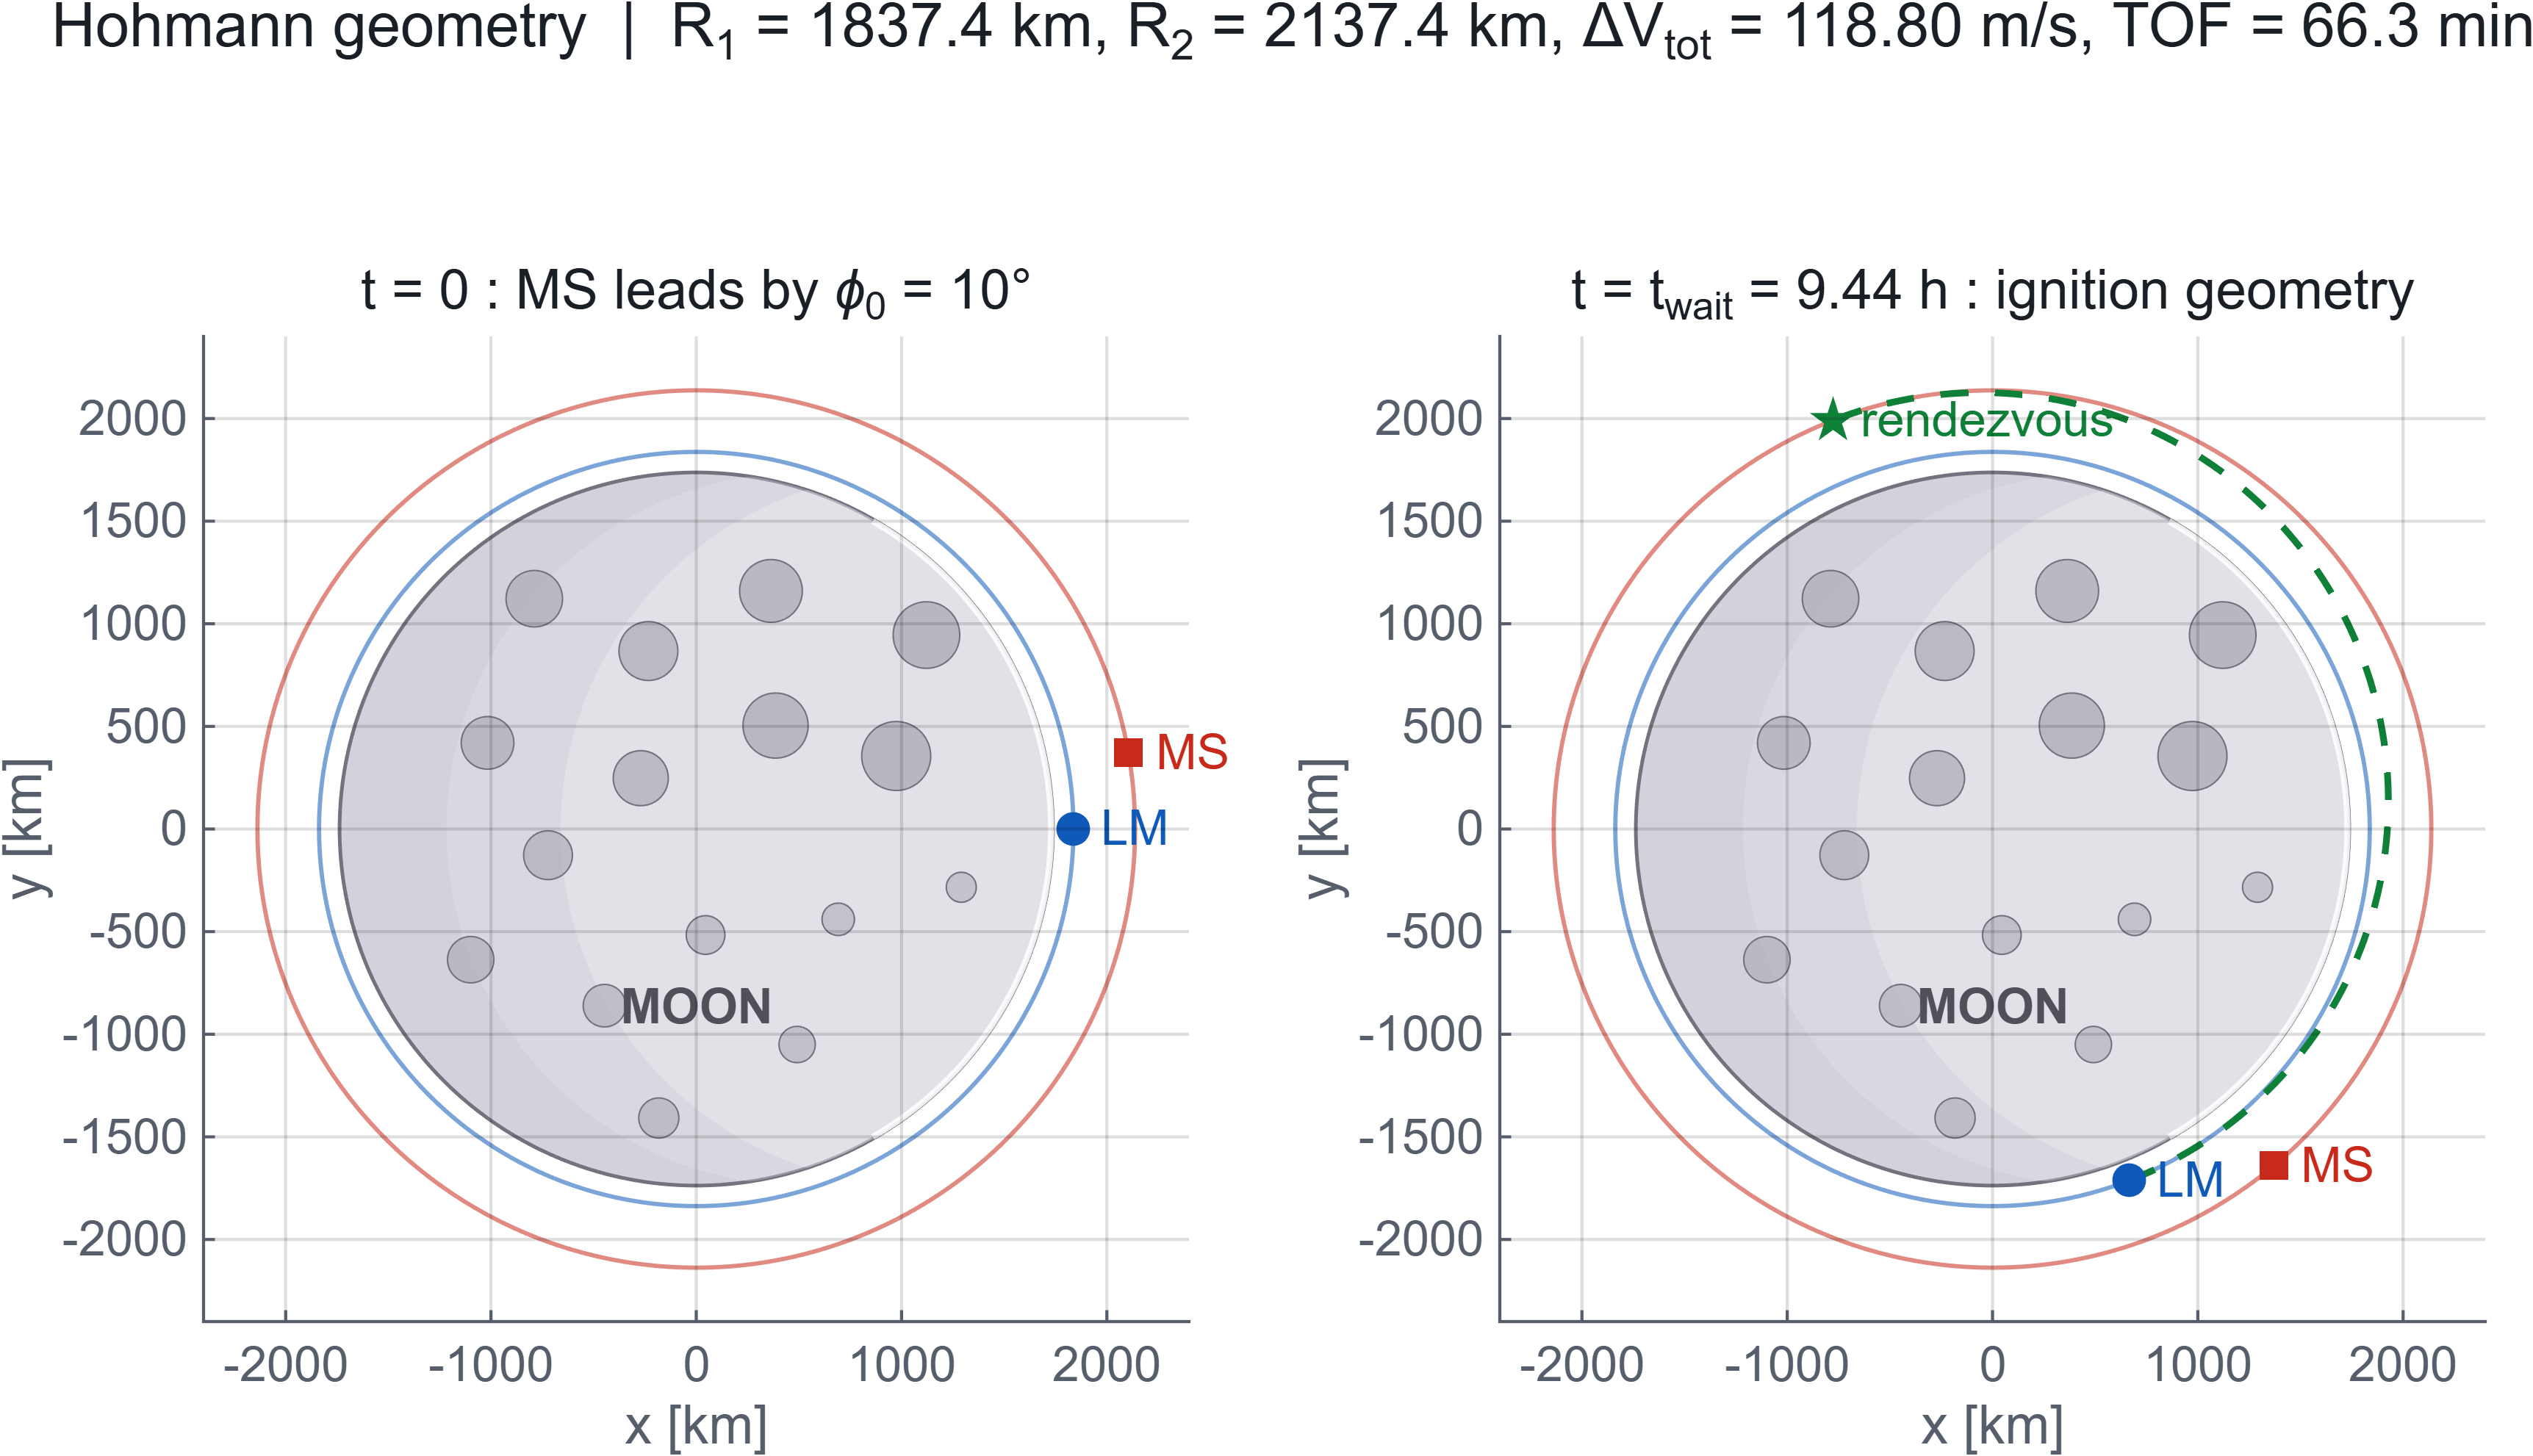
\includegraphics[width=\textwidth]{fig02_hohmann_geometry.png}
\caption{Transfer geometry at the epoch (left) and at ignition (right). The
target leads by $10^\circ$ at $t=0$ but the manoeuvre needs $\mLeadDeg^\circ$,
so the chaser coasts $\mTwaitH$ hours on the inner orbit before the burn. The
dashed ellipse is the $\mDVtot\unit{m/s}$ transfer.}
\label{fig:geometry}
\end{figure}

\subsection{Numerical propagation}

The full timeline is integrated in Cartesian coordinates with the unperturbed
two-body field,

\begin{equation}
\dot{\mathbf r} = \mathbf v, \qquad
\dot{\mathbf v} = -\mu_M \frac{\mathbf r}{\lVert \mathbf r \rVert^3},
\label{eq:twobody}
\end{equation}

using \texttt{ode45} at relative and absolute tolerances of $10^{-12}$. At
$t = t_{\text{wait}}$ the departure impulse is applied along the instantaneous
velocity unit vector; at apoapsis the second impulse circularises the orbit so
that the constants of motion display a third plateau.

\subsection{Verification against the closed-form solution}
\label{sec:transfer:verif}

The same timeline is then evaluated analytically and differenced. Circular legs
are trivial. On the transfer ellipse the mean anomaly $M = n_H (t - t_{\text{wait}})$
is inverted for the eccentric anomaly by Newton--Raphson,

\begin{equation}
E_{k+1} = E_k - \frac{E_k - e\sin E_k - M}{1 - e\cos E_k},
\label{eq:kepler}
\end{equation}

iterated to $10^{-14}$, and the perifocal state

\begin{equation}
\mathbf r_{pf} = \begin{bmatrix} a(\cos E - e) \\ a\sqrt{1-e^2}\,\sin E \\ 0 \end{bmatrix}
\label{eq:perifocal}
\end{equation}

is rotated into MCI by $R_z(\theta_p)$, with $\theta_p$ the ignition longitude.

Over the whole $\mTmissionH\unit{h}$ timeline the two solutions differ by at most
$\mKeplerErrMm\unit{mm}$ in position, and the numerically propagated rendezvous
closes to $\mMissKep\unit{m}$. This is the single most important number in the
report: it is the licence to believe every perturbed result that follows.

\paragraph{Two different quantities, two different names.}
The millimetre-class figure above is an \emph{integrator residual}: the largest
difference between the \texttt{ode45} state and the closed-form Kepler state at
the same epochs, stored as \texttt{miss\_num\_vs\_kepler}. It is not the
vehicle-to-vehicle separation quoted for the unperturbed control case in
Table~\ref{tab:miss}, which is $\mMissTwoBody\unit{m}$ and is stored as
\texttt{miss\_LM\_MS\_twobody}. That one is an LM--MS distance produced by the
Section~\ref{sec:perturbations} Cowell pipeline with the perturbations switched
off, so it carries that pipeline's working tolerance and both impulse
applications, not the propagator alone. Both are small, they are allowed to
differ by two orders of magnitude, and quoting one for the other would be
wrong. Earlier drafts of this report did exactly that.
When Section~\ref{sec:perturbations} reports a $\mMissJtwo\unit{km}$ miss under
$J_2$, we know that $15\unit{km}$ is physics and not integrator drift, because
the same integrator reproduces the analytical solution to a fifth of a
millimetre.

\begin{figure}[htbp]
\centering
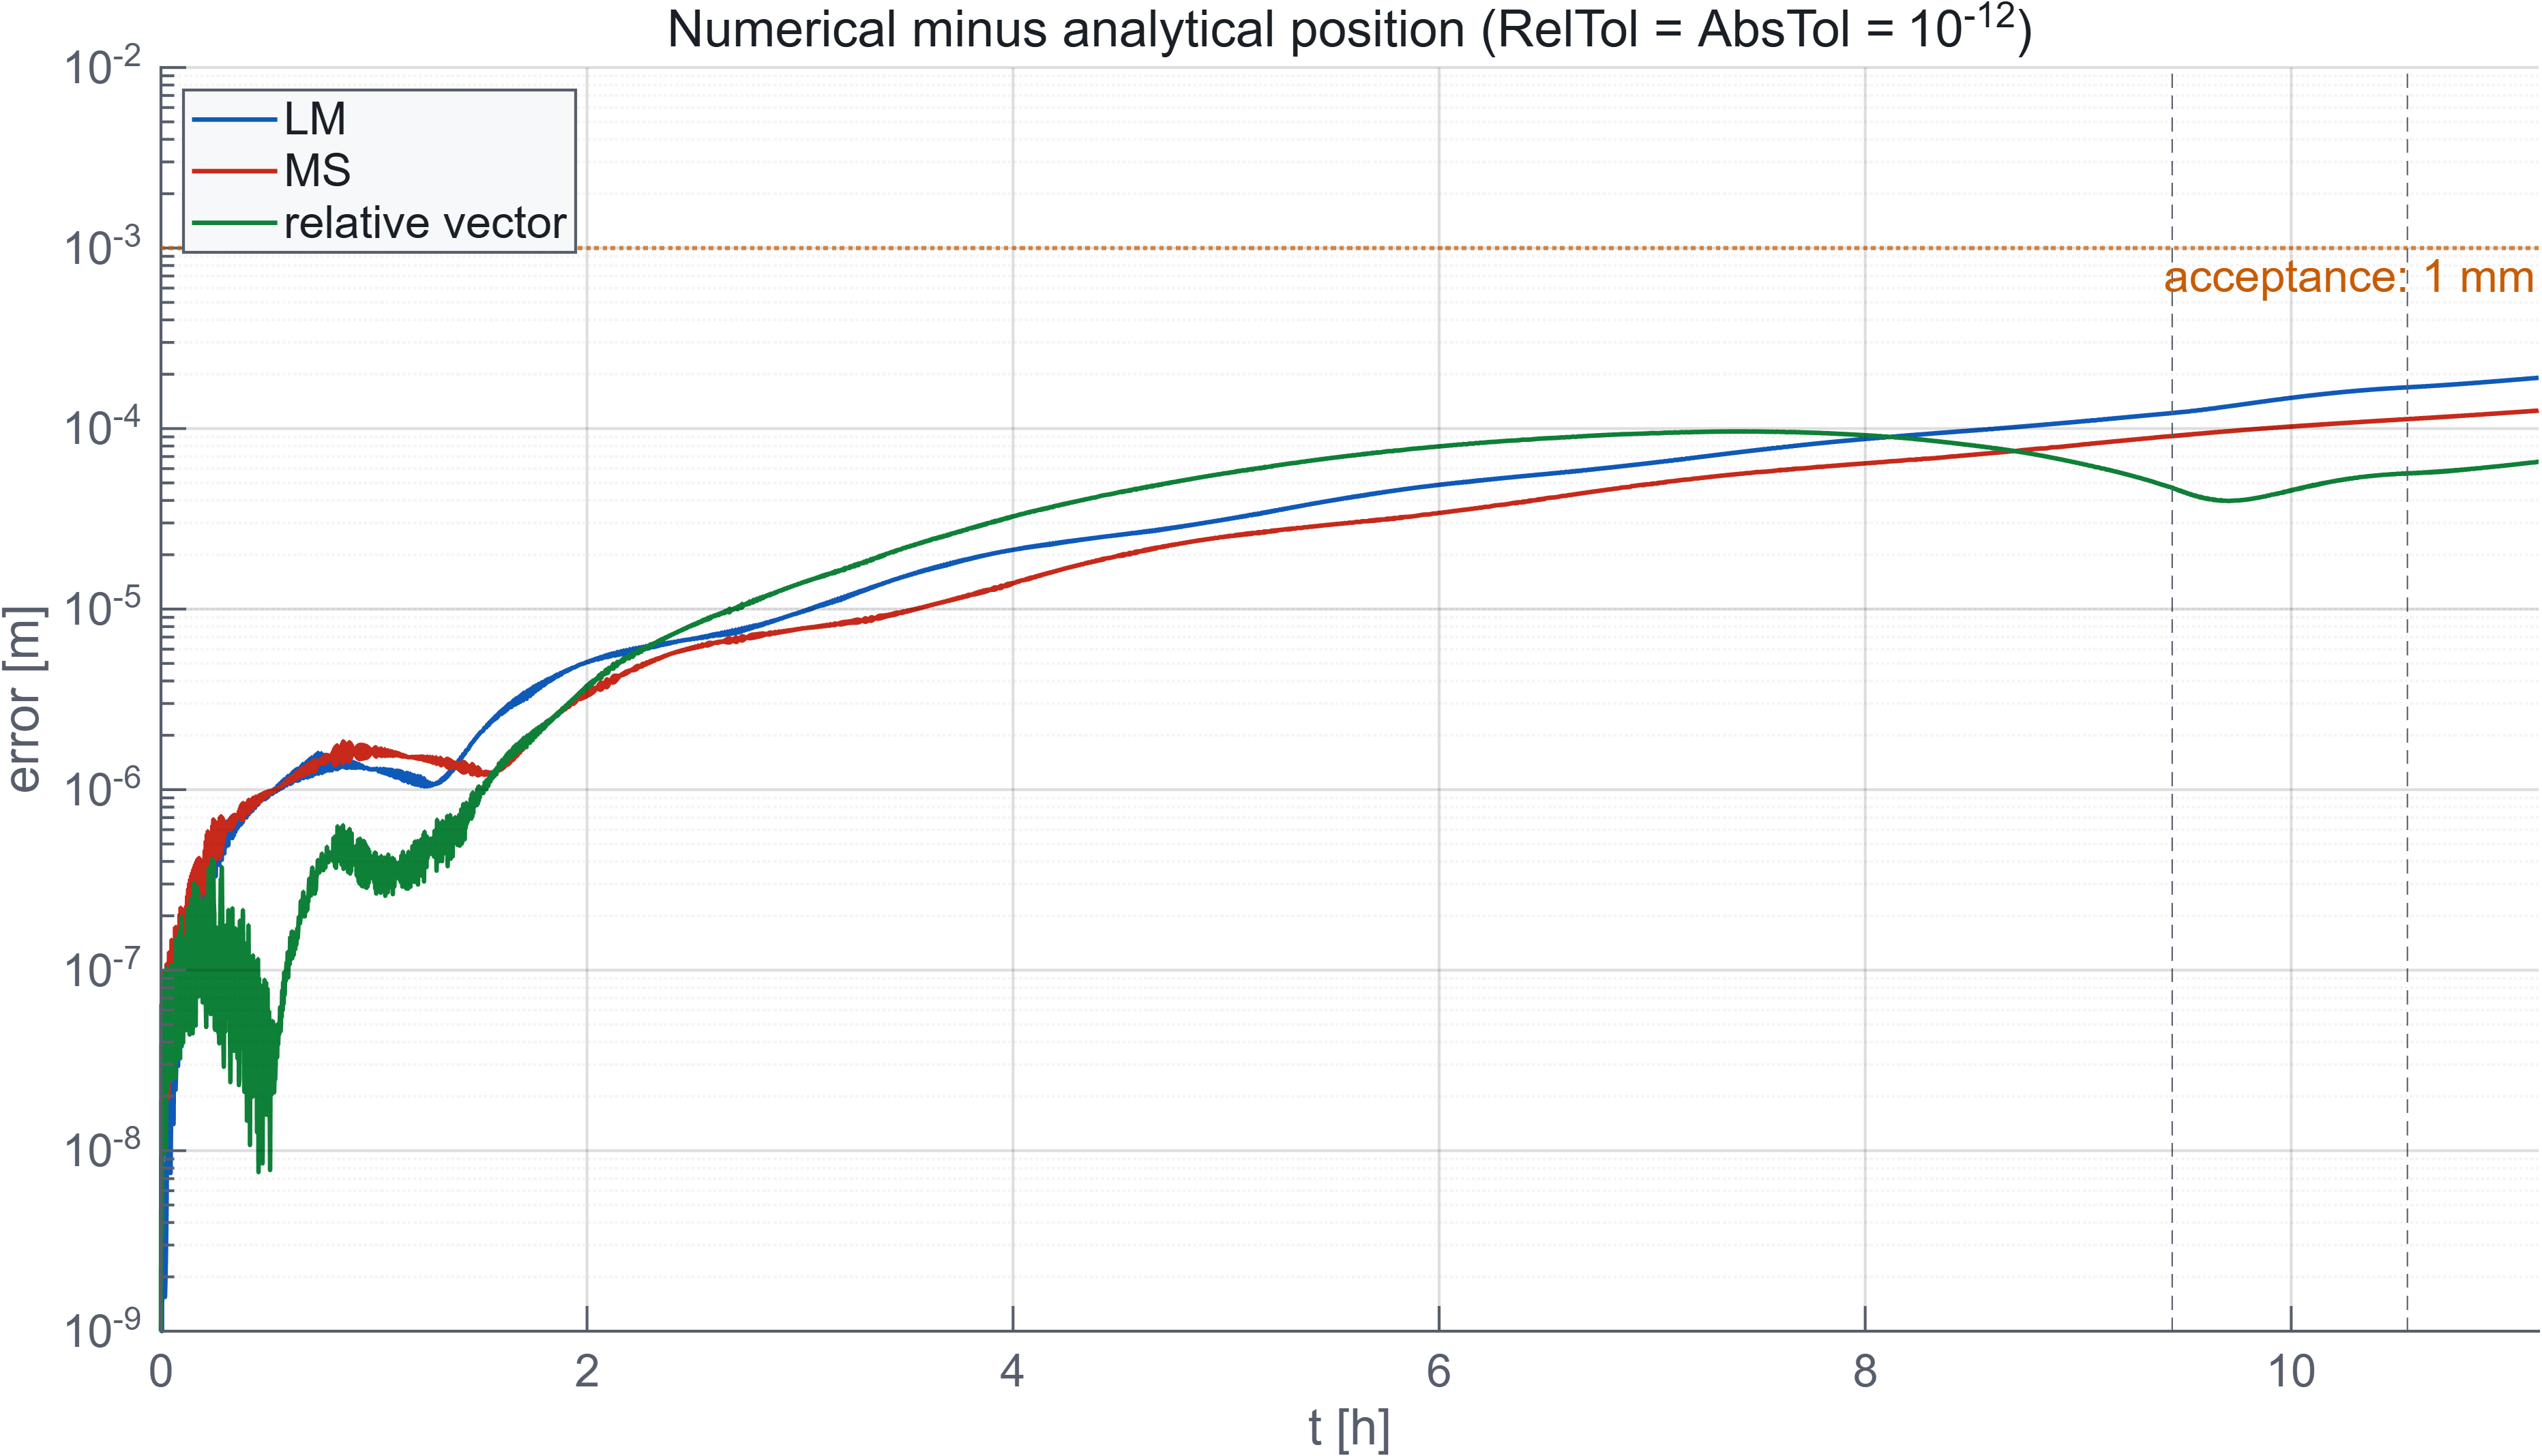
\includegraphics[width=0.93\textwidth]{fig04_position_errors.png}
\caption{Difference between the \texttt{ode45} solution and the closed-form
Kepler solution over the full timeline, log scale. The error grows smoothly to
$\mKeplerErrMm\unit{mm}$, three orders of magnitude below the $1\unit{mm}$
acceptance line. Dashed verticals mark the two impulses.}
\label{fig:keplererr}
\end{figure}

\subsection{Constants of motion}

For a further independent check the specific energy, angular momentum and
eccentricity vector are evaluated along the trajectory,

\begin{equation}
\varepsilon = \frac{v^2}{2} - \frac{\mu_M}{r}, \qquad
\mathbf h = \mathbf r \times \mathbf v, \qquad
\mathbf e = \frac{1}{\mu_M}\!\left[\left(v^2 - \frac{\mu_M}{r}\right)\mathbf r - (\mathbf r \cdot \mathbf v)\mathbf v\right].
\label{eq:constants}
\end{equation}

These must be piecewise constant, stepping only at the two impulses.
Table~\ref{tab:constants} compares the simulated plateaus with the closed-form
values $\varepsilon = -\mu_M/2a$ and $\lVert\mathbf h\rVert = \sqrt{\mu_M a(1-e^2)}$;
they agree to twelve significant figures.

\begin{table}[htbp]
\centering
\caption{Constants of motion per leg. Analytical and simulated values agree to
better than $10^{-12}$ relative, confirming that the impulses are applied
cleanly and that no energy leaks through the integrator.}
\label{tab:constants}
\small
\begin{tabular}{lrrr}
\toprule
Leg & $e$ & $\lVert\mathbf h\rVert$ [km$^2$/s] & $\varepsilon$ [km$^2$/s$^2$] \\
\midrule
Inner circular   & $0$      & $3001.40$ & $-1.33417$ \\
Transfer ellipse & $\mEcc$  & $3112.61$ & $-1.23347$ \\
Outer circular   & $0$      & $3237.17$ & $-1.14691$ \\
\bottomrule
\end{tabular}
\end{table}

\clearpage
\section{Relative dynamics and proximity operations}
\label{sec:proximity}

\subsection{The injection error is the whole point}

The rendezvous of Section~\ref{sec:transfer} closes to a fraction of a
millimetre, which no ascent stage has ever achieved. The dispersion listed in
Section~1.1 -- single-string propulsion, thrust-to-centre-of-mass misalignment,
active-only attitude control, migrating inertia -- arrives at the top of the
climb as a position and velocity offset. This part models that offset explicitly
and prices its removal.

The error is drawn once from a seeded generator: a random direction with
magnitude uniform in $[500, 1000]\unit{m}$ for position and $[0.1, 1]\unit{m/s}$
for velocity. The realisation used throughout is
$\lVert\delta\mathbf r_0\rVert = \mDrZero\unit{m}$ and
$\lVert\delta\mathbf v_0\rVert = \mDvZero\unit{m/s}$. The seed, not the numbers,
is the reproducibility mechanism.

\subsection{Frame definition, and the sign trap inside it}
\label{sec:proximity:frame}

Relative motion is expressed in a local frame attached to the target. This
report uses

\begin{equation}
\hat{\mathbf x} = -\hat{\mathbf v}, \qquad
\hat{\mathbf y} = -\hat{\mathbf h}, \qquad
\hat{\mathbf z} = +\hat{\mathbf r},
\label{eq:lvlh}
\end{equation}

that is, $x$ along the \vbar{} measured positive \emph{astern} of the target,
$y$ cross-track along the negative orbit normal, and $z$ along the \rbar{},
positive outward. The triad is right-handed, since
$\hat{\mathbf x}\times\hat{\mathbf y} = (-\hat{\mathbf v})\times(-\hat{\mathbf h})
= \hat{\mathbf v}\times\hat{\mathbf h} = \hat{\mathbf r}$.

\begin{quote}\small\itshape
\textbf{This is not Fehse's frame.} Fehse's $+$\vbar{} points ahead of the
target; here it points astern. A ``$50\unit{m}$ \vbar{} hold'' in this report is
therefore $50\unit{m}$ \emph{behind} the target, and the sign of every Coriolis
term below is flipped relative to Fehse or to any radial/along-track
formulation. Every number in Part~3 is internally consistent with this choice.
They are not interchangeable with a Fehse implementation without negating $x$
and $\dot x$. Reference~\cite{fehse} is cited for the linearisation and for the
operational shape of the approach, not as the source of this axis convention.
\end{quote}

Two remarks justify what looks at first like a perverse choice. Operationally,
\vbar{} range is quoted astern: a ``$50\unit{m}$ \vbar{} hold'' is $50\unit{m}$
behind the target, and the approach then walks $x$ from $+50\unit{m}$ down to
zero at the port. Mathematically, the price is that the target's angular
velocity is $-n$ about the frame's own $y$ axis, which flips the sign of every
Coriolis term relative to the textbook radial/along-track ordering. Linearising
about a circular chief \cite{cw1960} gives

\begin{align}
\ddot x - 2n\dot z &= 0, \label{eq:hcw1}\\
\ddot y + n^2 y &= 0, \label{eq:hcw2}\\
\ddot z + 2n\dot x - 3n^2 z &= 0. \label{eq:hcw3}
\end{align}

This is exactly where a sign error hides most comfortably: copy a state
transition matrix written for $x$ radial, label the axes \vbar{} and \rbar{}, and
the free-drift plot still looks plausible while every targeting solution is
quietly wrong. The convention was therefore settled empirically rather than
asserted, and it is now pinned by \texttt{tests/test\_hcw\_convention.m}, which
checks $\Phi(0) = I$, $\Phi(t)\Phi(-t) = I$, $\dot\Phi(0) = A$, the closed form
against a column-by-column numerical integration of the same linear system to
$3\times10^{-9}$, the sign and magnitude of the radial-release drift, and the
reference cross-check below.

Fed an independent implementation's injection error, the targeting of
Section~\ref{sec:proximity:hold} returns $1.419\unit{m/s}$ against that
implementation's $1.4\unit{m/s}$. Reading the same physical state in the
ahead-positive frame instead returns $1.236\unit{m/s}$ and does not reproduce
it. That is the evidence for the frame, and it is also why the ahead-positive
convention was not adopted: switching would have broken the only independent
check Part~3 has.

A physical check completes the argument. Release the chaser $100\unit{m}$
radially outward at zero relative velocity: it is on a higher, slower orbit and
must fall behind. The state transition matrix returns $x = +11.3\unit{km}$ after
three orbits, and since $+x$ is astern, it has indeed fallen behind. Reading
$+x$ as ``ahead'' is the trap; the sign is correct once the axis direction is
stated.

\subsection{State transition matrix}

With $\tau = nt$ and the state $\delta\mathbf x = [x\ y\ z\ \dot x\ \dot y\ \dot z]^\top$,
equations~\eqref{eq:hcw1}--\eqref{eq:hcw3} integrate in closed form to
$\delta\mathbf x(t) = \Phi(t)\,\delta\mathbf x(0)$ with

\begin{equation}
\Phi(t) =
\begin{bmatrix}
1 & 0 & 6(\tau-\sin\tau) & \frac{4\sin\tau-3\tau}{n} & 0 & \frac{2(1-\cos\tau)}{n}\\[2pt]
0 & \cos\tau & 0 & 0 & \frac{\sin\tau}{n} & 0\\[2pt]
0 & 0 & 4-3\cos\tau & \frac{2(\cos\tau-1)}{n} & 0 & \frac{\sin\tau}{n}\\[2pt]
0 & 0 & 6n(1-\cos\tau) & 4\cos\tau-3 & 0 & 2\sin\tau\\[2pt]
0 & -n\sin\tau & 0 & 0 & \cos\tau & 0\\[2pt]
0 & 0 & 3n\sin\tau & -2\sin\tau & 0 & \cos\tau
\end{bmatrix}.
\label{eq:stm}
\end{equation}

Three properties are checked automatically: $\Phi(0) = I$ to machine precision;
$\dot\Phi(0)$ equals the system matrix of the first-order form, which is what
actually pins the Coriolis signs; and $\Phi(t)\Phi(-t) = I$.

\subsection{Free drift}

Propagating the injection error with no correction is instructive.
Figure~\ref{fig:drift} shows the result over three target orbits: the
out-of-plane component is a bounded harmonic at the orbital frequency, while the
in-plane motion develops a secular along-track drift driven by the period
mismatch. The separation reaches $\mDriftKm\unit{km}$.

That number is the argument for active proximity operations in one line. A
$0.88\unit{m/s}$ velocity error, roughly $0.05\%$ of orbital speed, becomes a
$21\unit{km}$ miss within seven hours.

\begin{figure}[htbp]
\centering
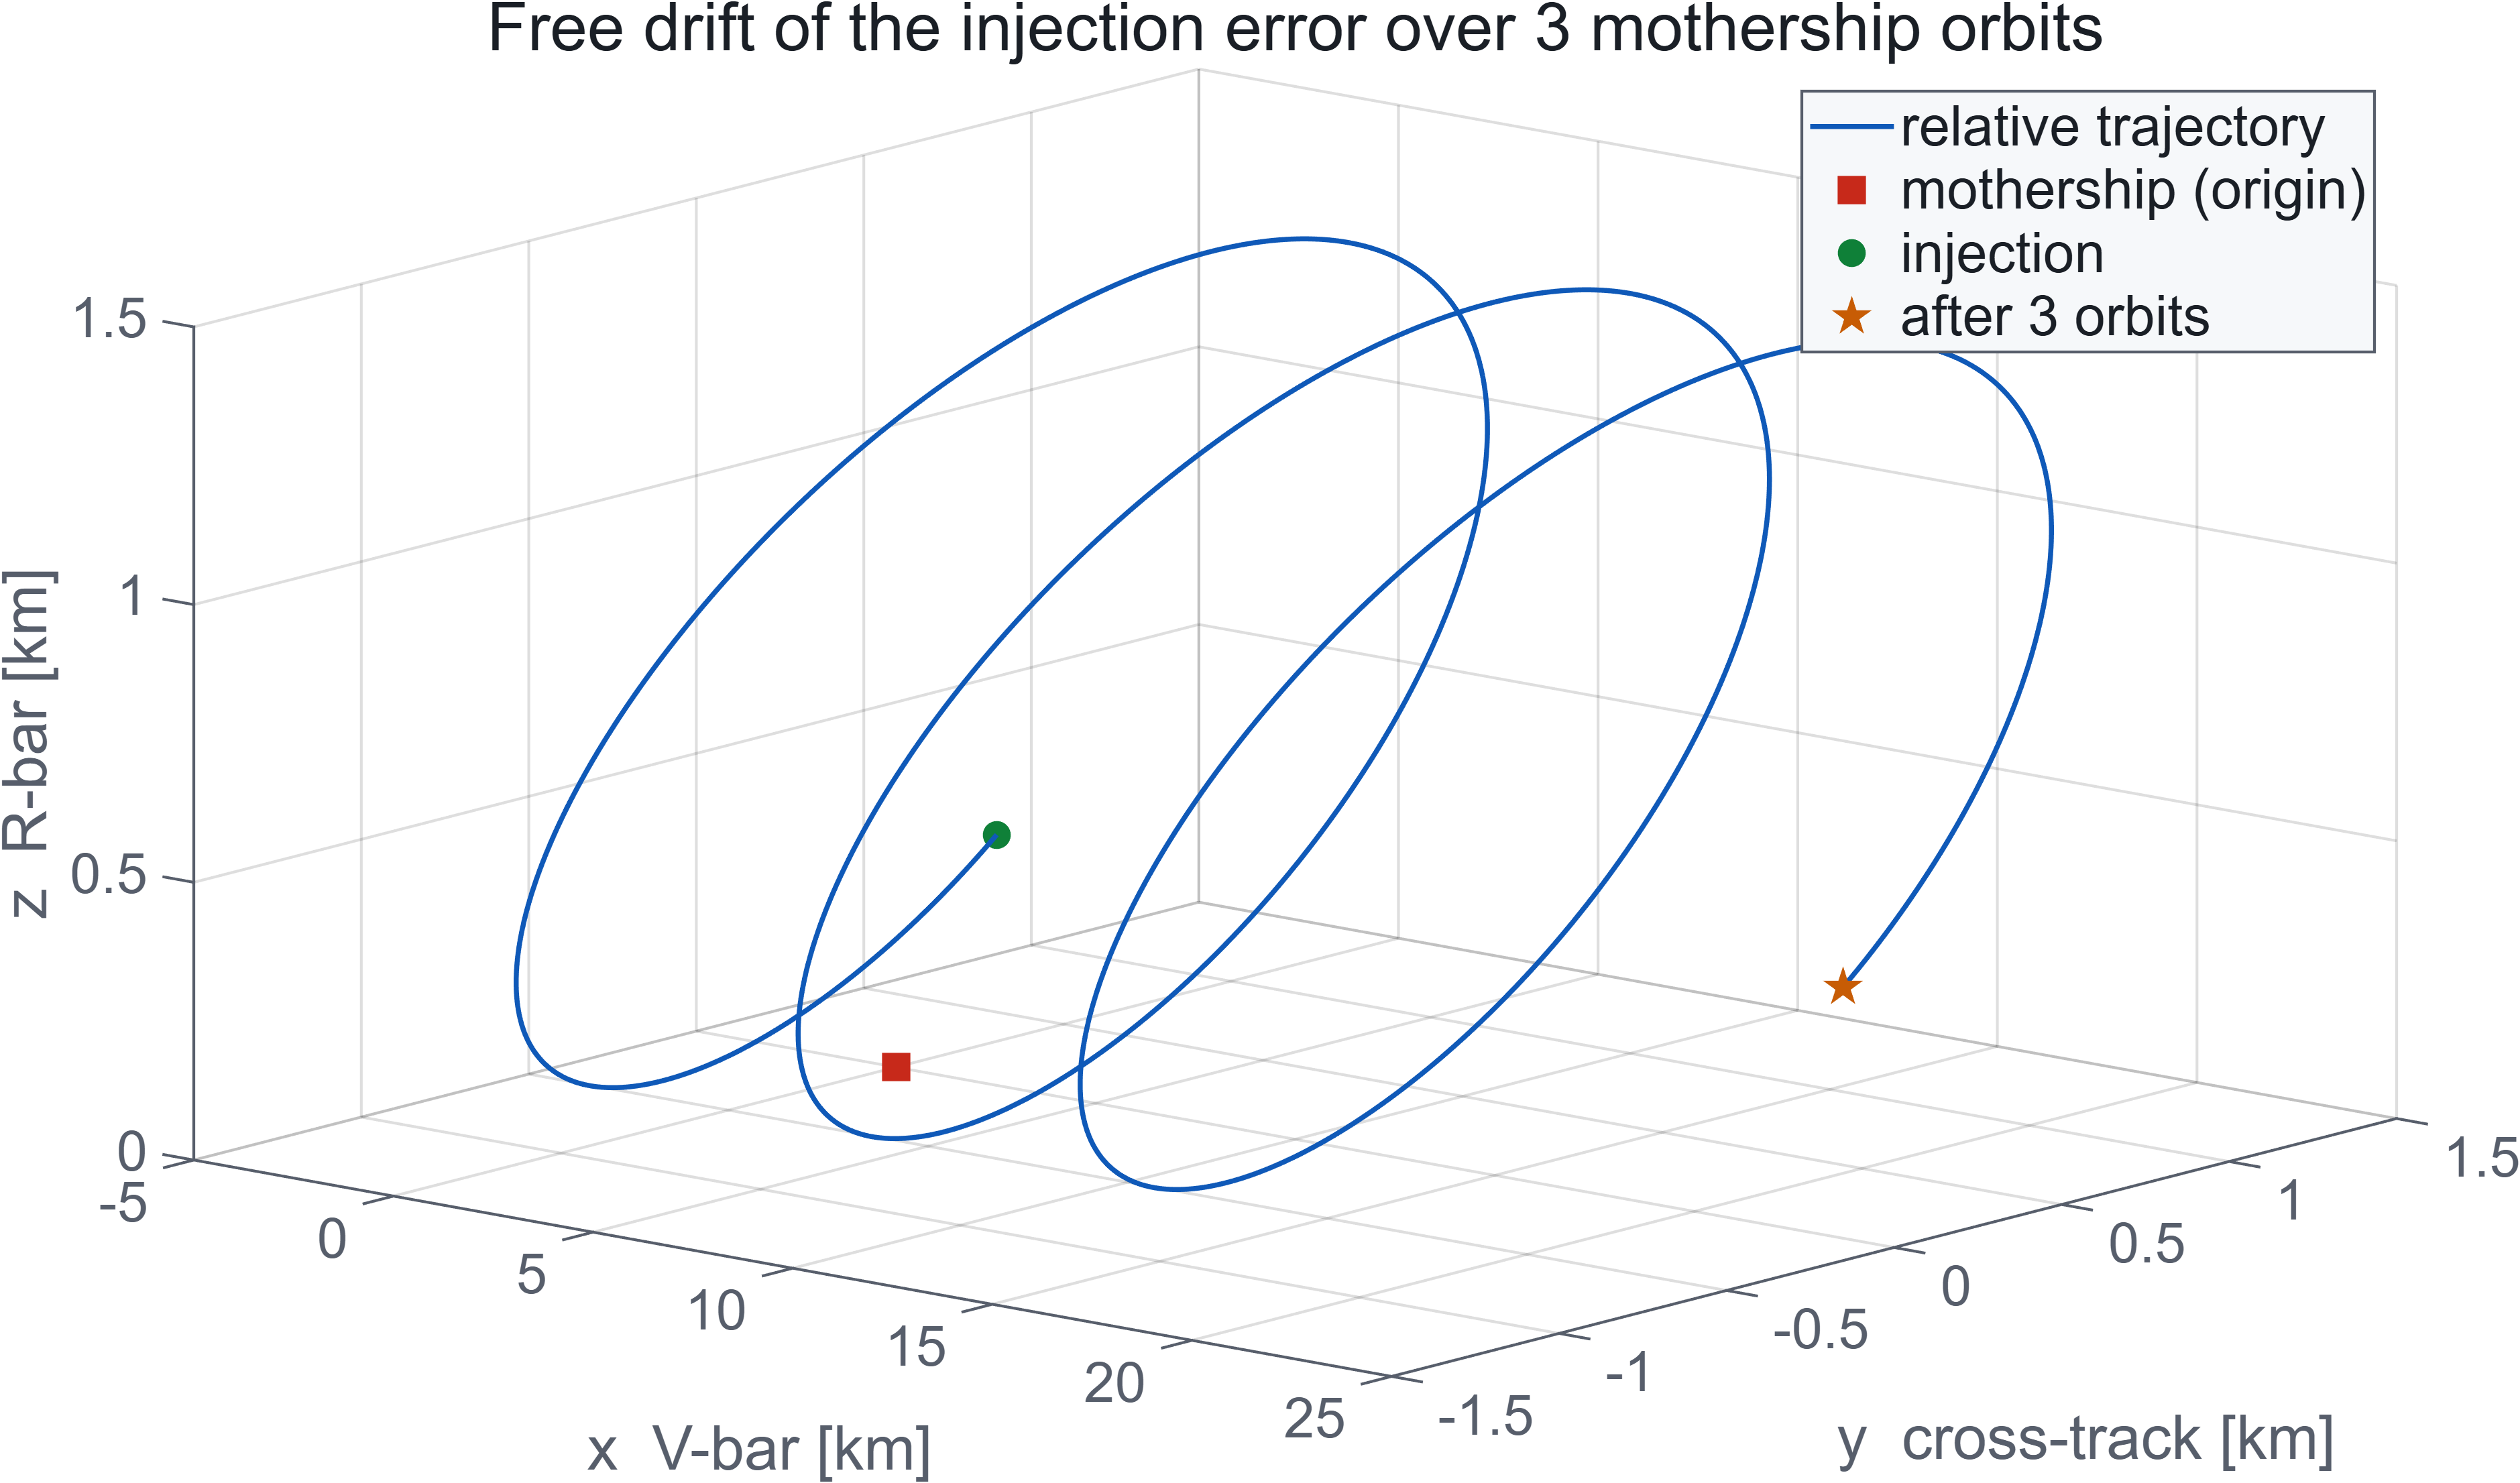
\includegraphics[width=0.78\textwidth]{fig06_free_drift_3d.png}
\caption{Uncorrected injection error over three target orbits in the local
frame. Starting from $\mDrZero\unit{m}$ and $\mDvZero\unit{m/s}$, the chaser
drifts $\mDriftKm\unit{km}$ along-track. Cross-track motion stays bounded.}
\label{fig:drift}
\end{figure}

\subsection{Two-impulse hold acquisition}
\label{sec:proximity:hold}

Partitioning~\eqref{eq:stm} into $3\times3$ blocks, the transfer from the
injection state to a prescribed hold point in a prescribed time is a single
linear solve:

\begin{equation}
\mathbf v_0^+ = \Phi_{rv}^{-1}\!\left(\mathbf r_{\text{hold}} - \Phi_{rr}\,\delta\mathbf r_0\right),
\qquad
\dv_1 = \mathbf v_0^+ - \delta\mathbf v_0,
\label{eq:target1}
\end{equation}
\begin{equation}
\dv_2 = \mathbf v_{\text{hold}} - \left(\Phi_{vr}\,\delta\mathbf r_0 + \Phi_{vv}\,\mathbf v_0^+\right).
\label{eq:target2}
\end{equation}

The hold point is $\mathbf r_{\text{hold}} = [50, 0, 0]^\top\unit{m}$ and the
transfer time $0.3\,T_{MS} = \mDtTr\unit{s}$. The cost is
$\dv_{\text{hold}} = \mDVhold\unit{m/s}$, and propagating the resulting
two-burn trajectory back through~\eqref{eq:stm} arrives within
$10^{-13}\unit{m}$ of the target point.

The block $\Phi_{rv}$ becomes singular whenever the transfer time approaches a
multiple of the orbital period, because after a full revolution the initial
velocity no longer controls the final position. Its condition number is
therefore checked before every solve and the transfer time nudged by $1\%$ until
the inversion is safe; at $0.3\,T_{MS}$ the reciprocal condition number is
$0.21$, comfortably clear.

\subsection{Forced straight-line \vbar{} approach}

From the hold point the vehicle is walked to the port in $N = 5$ equal legs of
$200\unit{s}$, each targeting the waypoint
$\mathbf r_k = \mathbf r_{\text{hold}}(1 - k/N)$, followed by a braking impulse
that nulls the residual velocity at contact. The total is
$\dv_{\text{dock}} = \mDVdock\unit{m/s}$, and the trajectory terminates
$3\times10^{-16}\unit{m}$ from the origin.

This profile is not chosen for elegance. A sequence of short targeted hops keeps
plume impingement away from the target, bounds the closing rate between
checkpoints, and gives the crew or the ground a natural abort opportunity at
every waypoint -- the pattern used on real \vbar{} approaches \cite{fehse}.

\begin{figure}[htbp]
\centering
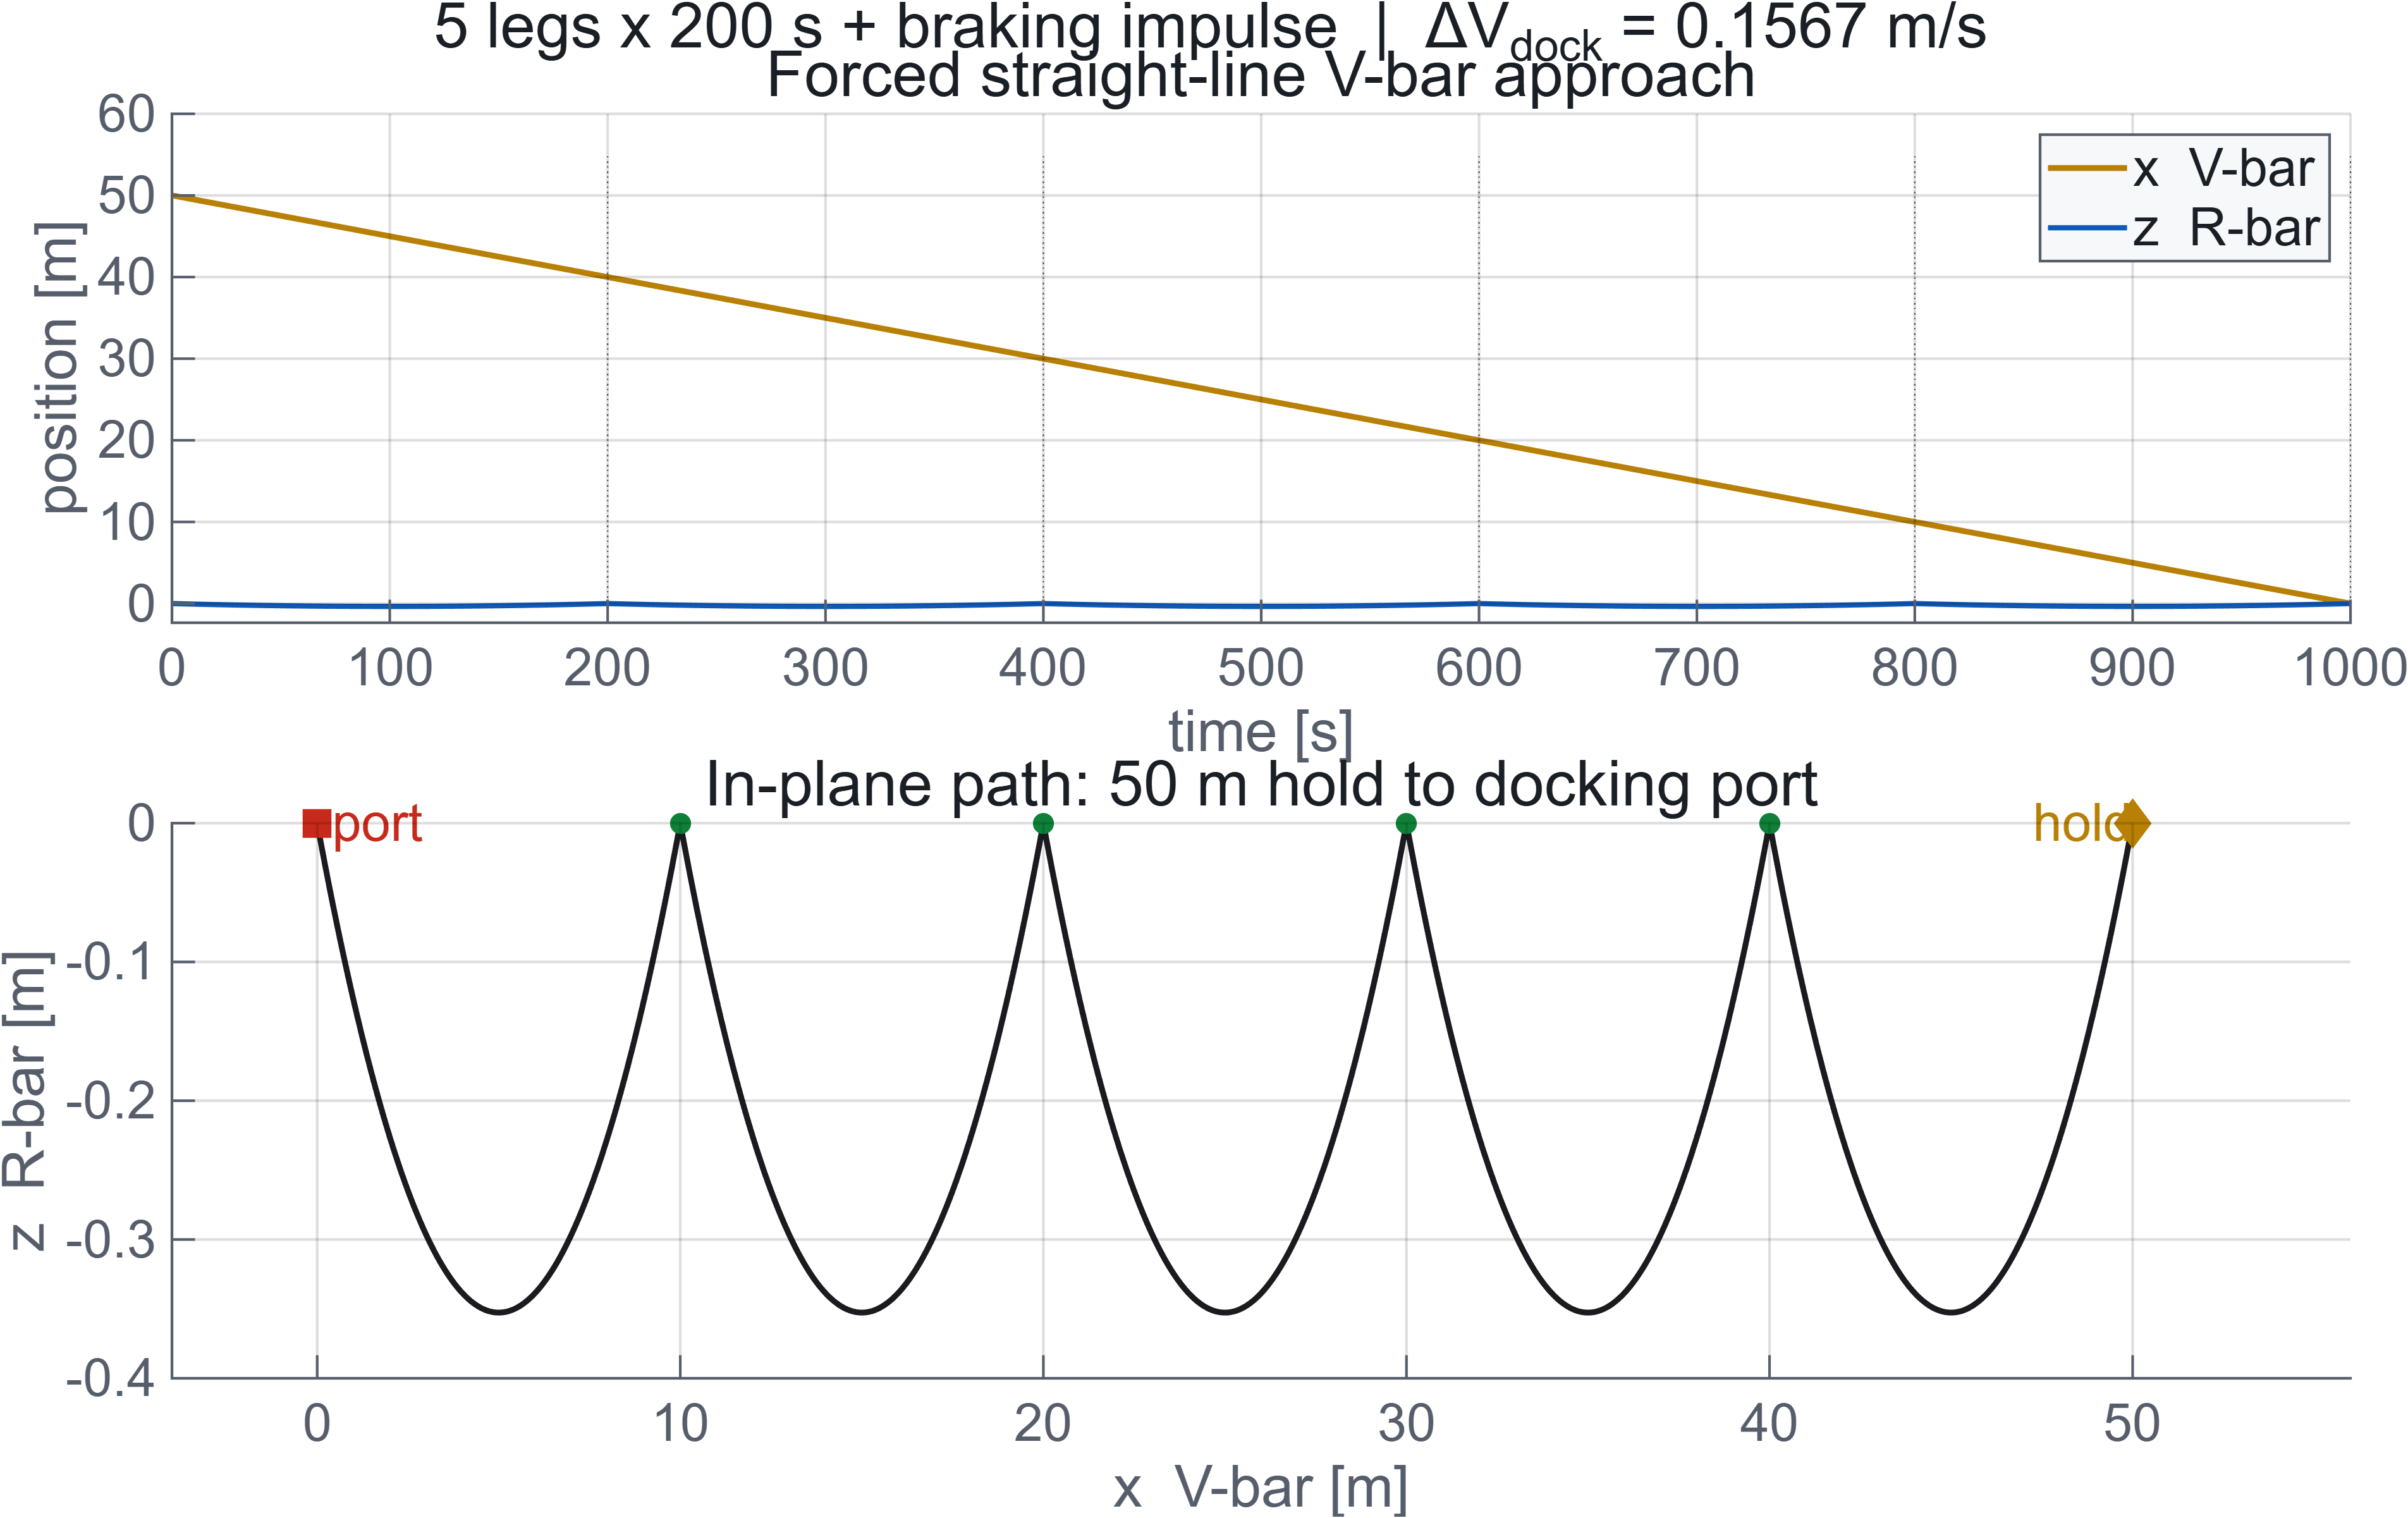
\includegraphics[width=0.93\textwidth]{fig08_forced_vbar_docking.png}
\caption{Forced straight-line approach. Top: \vbar{} and \rbar{} components
against time, with the six impulses marked. Bottom: the in-plane path from the
$50\unit{m}$ hold to the docking port, total cost $\mDVdock\unit{m/s}$.}
\label{fig:docking}
\end{figure}

The full proximity phase therefore costs $\mDVprox\unit{m/s}$, about $1\%$ of
the $\mDVtot\unit{m/s}$ transfer budget. That is the price of the ascent
dispersion, and it is only obtainable by modelling both phases in the same
units.

\subsection{Verification against the nonlinear equations}

The linear model is finally checked against the exact nonlinear relative
equations of motion for a circular chief, integrated with the same tolerances.
Writing $\rho^2 = x^2+y^2+z^2$ and $r_c = \sqrt{x^2+y^2+(R_2+z)^2}$, and using
the regularised form

\begin{equation}
q = \frac{\rho^2 + 2R_2 z}{R_2^2}, \qquad
F = \frac{q\left(2 + q + \sqrt{1+q}\right)}{(1+q)^{3/2}\left(1+\sqrt{1+q}\right)},
\label{eq:nonlin}
\end{equation}

avoids differencing two nearly equal inverse cubes, which matters when
$\rho/R_2 \sim 10^{-5}$.

The two models part company by $\mNlSep\unit{m}$ after three orbits at kilometre
range -- about half a percent of the separation. At the $50\unit{m}$ hold point,
where $\rho/R_2 = 2.3\times10^{-5}$, they agree to well under a millimetre. The
linearisation is used exactly where it is valid, and the divergence at long
range is quantified rather than assumed away.

\clearpage
\section{Perturbed dynamics}
\label{sec:perturbations}

\subsection{Purpose of the experiment}

Sections~\ref{sec:transfer} and~\ref{sec:proximity} live in a pure two-body
field. This part asks a specific operational question: if the manoeuvre plan is
designed in that field and flown against a more complete one \emph{without
retargeting}, how far off does it arrive? The answer sizes the mid-course
correction that a real flight plan must carry.

\subsection{Cowell formulation}

Perturbations are added directly to the acceleration in Cartesian coordinates,

\begin{equation}
\ddot{\mathbf r} = -\mu_M\frac{\mathbf r}{r^3}
                 + \mathbf a_{J_2}
                 + \mathbf a_{3B}.
\label{eq:cowell}
\end{equation}

The oblateness term is the standard second zonal harmonic \cite{vallado},

\begin{equation}
\mathbf a_{J_2} = \frac{3 J_2 \mu_M R_M^2}{2 r^4}
\begin{bmatrix}
\dfrac{x}{r}\left(5\dfrac{z^2}{r^2}-1\right)\\[8pt]
\dfrac{y}{r}\left(5\dfrac{z^2}{r^2}-1\right)\\[8pt]
\dfrac{z}{r}\left(5\dfrac{z^2}{r^2}-3\right)
\end{bmatrix}.
\label{eq:j2}
\end{equation}

The full three-component expression is retained even though the orbits are
equatorial. At $z = 0$ it collapses correctly to a purely radial correction, so
special-casing it would add a branch and remove a check.

The Earth is included as a third body in Battin's difference form \cite{battin},

\begin{equation}
\mathbf a_{3B} = \mu_E\left(\frac{\mathbf r_E - \mathbf r}{\lVert \mathbf r_E - \mathbf r\rVert^3}
                          - \frac{\mathbf r_E}{\lVert \mathbf r_E \rVert^3}\right),
\label{eq:thirdbody}
\end{equation}

with the Earth on a circular path about the Moon at the synodic rate
$n_{EM} = \sqrt{(\mu_M+\mu_E)/d_{EM}^3}$. The second term is the indirect part:
it removes the acceleration of the origin, because the frame is Moon-centred and
the Moon is itself falling towards the Earth. Dropping it is a classic error
that inflates the computed effect by orders of magnitude; retaining it is what
makes the $116\unit{m}$ result of Section~\ref{sec:perturbations:results}
meaningful.

\subsection{Acceleration budget}

Before integrating anything it is worth knowing what matters.
Table~\ref{tab:accel} evaluates the characteristic magnitudes at the chaser's
orbit radius.

\begin{table}[htbp]
\centering
\caption{Characteristic accelerations at $r = R_1 = 1837.4\unit{km}$. Oblateness
dominates the perturbation budget by more than an order of magnitude over the
Earth, which in turn dominates radiation pressure by two.}
\label{tab:accel}
\small
\begin{tabular}{lrr}
\toprule
Source & Magnitude [m/s$^2$] & Ratio to central \\
\midrule
Central lunar attraction     & \mAkep  & $1$ \\
Lunar $J_2$                  & \mAJtwo & $2.7\times10^{-4}$ \\
Earth third body             & \mATB   & $1.8\times10^{-5}$ \\
Solar radiation pressure (estimated) & $\sim 10^{-7}$ & $\sim 7\times10^{-8}$ \\
\bottomrule
\end{tabular}
\end{table}

Radiation pressure is estimated rather than integrated. For an area-to-mass
ratio of order $0.01\unit{m^2/kg}$ and a reflectivity near $1.3$, the cannonball
acceleration at $1\unit{AU}$ is around $10^{-7}\unit{m/s^2}$. It is also
intermittent: a $100\unit{km}$ lunar orbit has a period near two hours and spends
roughly $30$--$40\%$ of each revolution in shadow, so the perturbation switches
on and off rather than accumulating smoothly. Integrated over the
$\mTmissionH\unit{h}$ mission the velocity change is of order
$10^{-3}\unit{m/s}$, three orders below the correction $J_2$ already demands.
The code carries a disabled flag for it and the omission is deliberate.

\subsection{Why an equatorial orbit still feels $J_2$}

For $z \equiv 0$ equation~\eqref{eq:j2} reduces to
$\mathbf a_{J_2} = -\tfrac{3}{2}J_2\mu_M R_M^2 r^{-5}\,[x, y, 0]^\top$: a purely
radial correction. It does not tilt the plane and it does not regress the node.
What it does is stiffen the central field by a \emph{radius-dependent} amount,

\begin{equation}
\frac{\delta a_r}{a_r} = \frac{3}{2} J_2 \left(\frac{R_M}{r}\right)^2,
\label{eq:j2ratio}
\end{equation}

which is $2.73\times10^{-4}$ at the chaser radius and $2.01\times10^{-4}$ at the
target radius, so the two vehicles accumulate \emph{different} along-track phase.
Over ten and a half hours that difference is kilometres, and the miss is
therefore almost purely along-track, which is what the simulation produces.

The size of that phase drift should be taken from the secular element rates
rather than from a stiffened-central-field argument. With
$\bar n = \sqrt{\mu_M/a^3}$, $p = a(1-e^2)$ and $k = \tfrac34 \bar n J_2 (R_M/p)^2$,
the classical first-order rates are \cite{vallado}

\begin{equation}
\dot\Omega = -2k\cos i, \qquad
\dot\omega = k\,(4 - 5\sin^2 i), \qquad
\dot M = \bar n + k\sqrt{1-e^2}\,(2 - 3\sin^2 i).
\label{eq:secular}
\end{equation}

On an equatorial circular orbit the node and the argument of periapsis are
individually undefined, but their sum with the mean anomaly is not. The
observable is the mean-longitude rate

\begin{equation}
\dot\lambda = \dot\Omega + \dot\omega + \dot M
            = \bar n\left[1 + 3 J_2 \left(\frac{R_M}{a}\right)^{\!2}\right],
\label{eq:lambdadot}
\end{equation}

an excess of $\mJtwoExcess$ at the chaser radius. Comparing~\eqref{eq:lambdadot}
with the slope of $\mathrm{unwrap}\,\arctan(y/x)$ taken from the $J_2$-only
Cowell arc gives agreement to $\mJtwoRateRel$ relative, which is the check
recorded in the audit.

It is worth noting what this replaces. An earlier draft argued that a stiffer
central field shifts the mean motion by $\delta n/n = \tfrac12\,\delta\mu_{\text{eff}}/\mu$,
giving an excess of $\tfrac34 J_2 (R_M/a)^2$. That captures only the radial
stiffening and drops the periapsis and node contributions, and it is a factor of
four too small. The numerical arc agrees with~\eqref{eq:lambdadot}, not with the
hand-wave.

\subsection{Results}
\label{sec:perturbations:results}

Both vehicles are propagated over the identical Part~1 timeline with the
identical perturbed dynamics; only their initial states differ. The departure
impulse keeps its Keplerian magnitude but is applied along the \emph{perturbed}
velocity unit vector sampled at $t_{\text{wait}}$, which is what an open-loop
vehicle would actually do. No retargeting is performed.

\begin{table}[htbp]
\centering
\caption{Rendezvous miss at the nominal arrival epoch, flying the Keplerian plan
against progressively more complete dynamics. The Keplerian control case through
the identical code path closes to $\mMissTwoBody\unit{m}$, so the residuals
below are physics and not integrator noise. That control number is a
vehicle-to-vehicle separation, not the $\mKeplerErrMm\unit{mm}$ propagator
residual of \S\ref{sec:transfer:verif}; the two are named separately in
\texttt{metrics.json}.}
\label{tab:miss}
\small
\begin{tabular}{lrl}
\toprule
Dynamics & Miss & Unit \\
\midrule
Two-body control case (\texttt{miss\_LM\_MS\_twobody}) & \mMissTwoBody & m \\
Lunar $J_2$                          & \mMissJtwo     & km \\
Lunar $J_2$ + Earth third body       & \mMissJtwoTB   & km \\
\midrule
Third-body contribution alone        & \mMissTB       & m \\
Mid-course correction, retargeted (\S\ref{sec:pert:mcc}) & \mMccReal & m/s \\
\bottomrule
\end{tabular}
\end{table}

\noindent
The control case is the LM--MS separation through this same pipeline with the
perturbations switched off. It is $\mMissTwoBody\unit{m}$, not the
$\mKeplerErrMm\unit{mm}$ integrator residual of \S\ref{sec:transfer:verif};
see the note there.

Three readings follow. First, oblateness alone moves the meeting point by
$\mMissJtwo\unit{km}$ -- far beyond any docking corridor, and the reason a real
plan carries a correction. Second, the Earth contributes only $\mMissTB\unit{m}$
of that: at $100$--$400\unit{km}$ altitude the vehicle is deep enough in the
lunar well that Earth tides are a hundred times smaller than lunar oblateness.
Third, the miss is cheap to remove if it is removed early: a retargeting
impulse placed halfway through the mission costs $\mMccReal\unit{m/s}$, well
under $1\%$ of the nominal transfer budget. Section~\ref{sec:pert:mcc} derives
that number and explains why the obvious estimate is an order of magnitude too
pessimistic.

\begin{figure}[htbp]
\centering
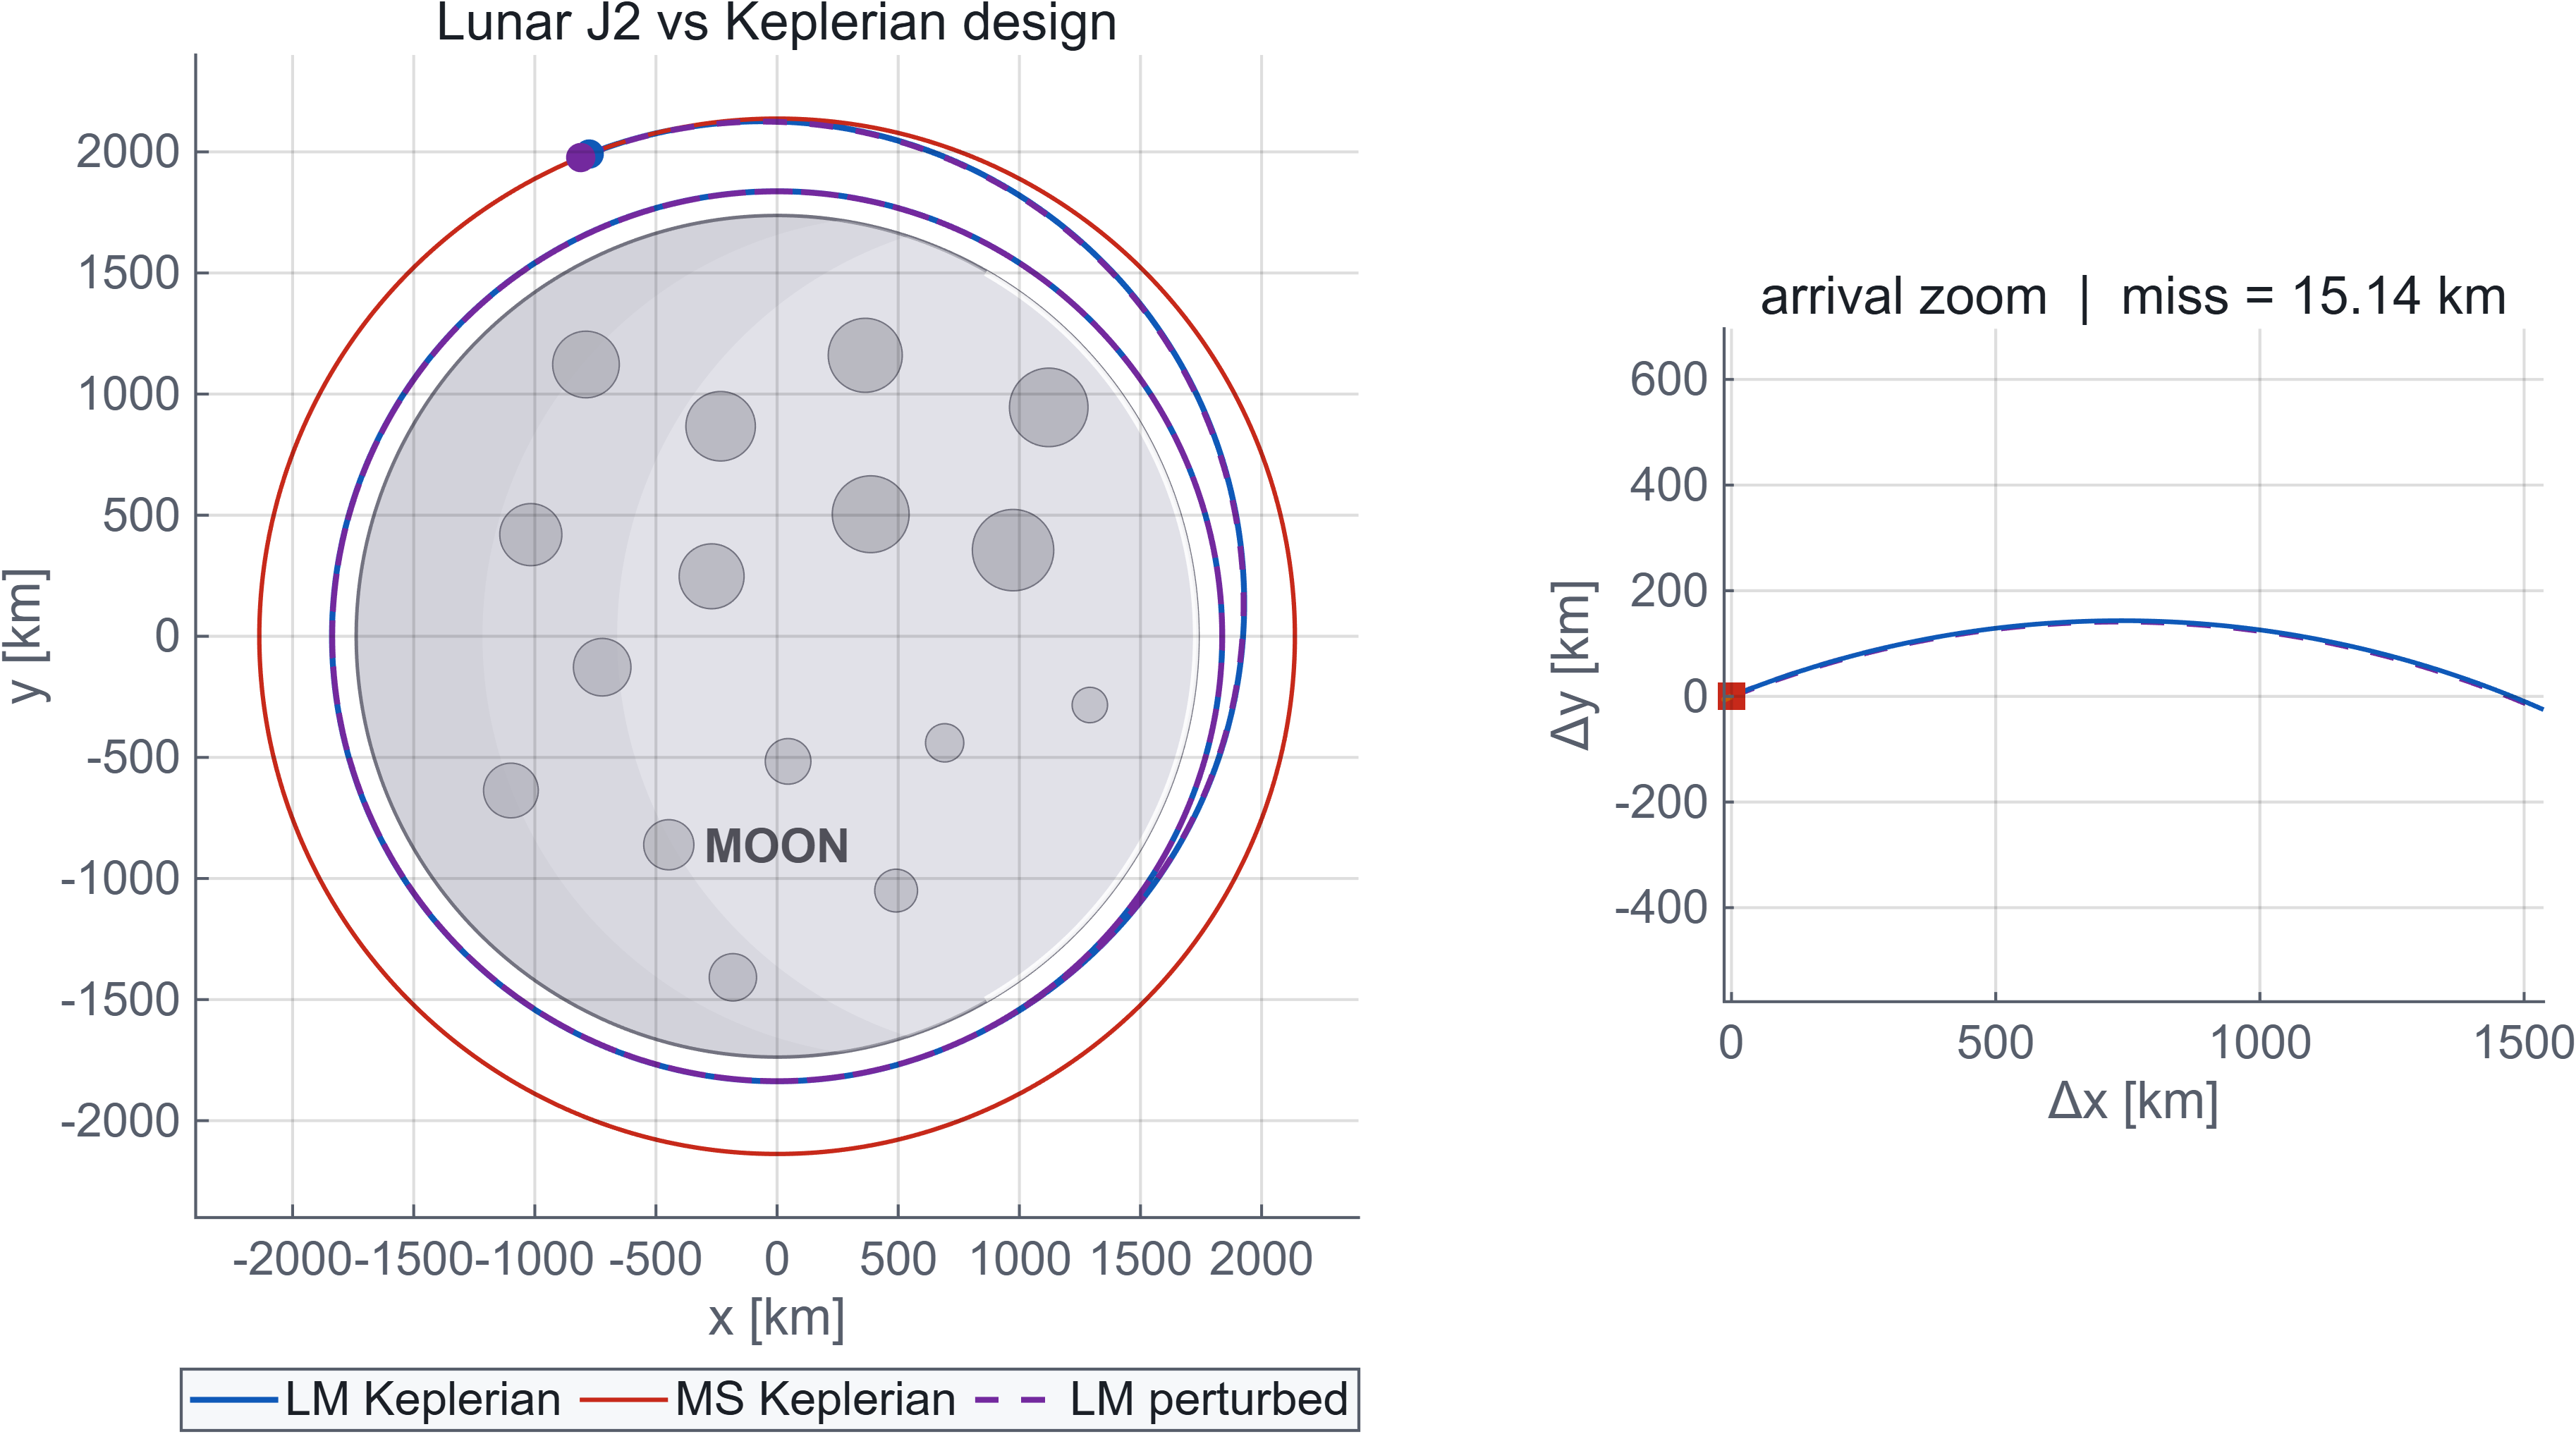
\includegraphics[width=\textwidth]{fig11_j2_vs_kepler.png}
\caption{Keplerian design (solid) against the same plan flown with lunar $J_2$
(dashed). The tracks are visually indistinguishable for ten hours; the inset
resolves the arrival neighbourhood, where the accumulated along-track phase slip
has become a $\mMissJtwo\unit{km}$ miss.}
\label{fig:j2}
\end{figure}

\subsection{Element histories}

Classical elements are extracted along the perturbed trajectories with a
degeneracy-safe conversion: the orbits are simultaneously circular and
equatorial, so both the node vector and the eccentricity vector vanish. The
implementation falls back on the true longitude, taking the node along $+x$ when
$\lVert\mathbf n\rVert$ is below a scale-aware threshold and folding the
argument of periapsis into the argument of latitude when $e < 10^{-8}$. Without
that guard the conversion returns noise for precisely the orbits this mission
uses.

\subsection{The mid-course correction, priced properly}
\label{sec:pert:mcc}

The tempting estimate is to treat the $\mMissJtwo\unit{km}$ offset as a
relative-motion problem and cancel it with a Clohessy--Wiltshire two-impulse
over a fraction of an orbit, which costs $n_2\lVert\mathbf d\rVert = \mMccNaive\unit{m/s}$.
That number is arithmetically correct and operationally wrong. Nobody flies a
$15\unit{km}$ along-track error as a proximity manoeuvre, because it is a
\emph{phase} error and phase is bought with time, not with thrust.

A $15\unit{km}$ along-track offset at $R_2$ is an angle of
$15/2137 \approx 7\unit{mrad}$. Correcting it with a small period change over
one target revolution needs

\begin{equation}
\Delta\theta = 3\pi\,\frac{\Delta a}{a}
\;\Longrightarrow\;
\frac{\Delta a}{a} \approx 7.5\times10^{-4}
\;\Longrightarrow\;
\Delta v \approx \tfrac12 n \Delta a \sim 0.6\unit{m/s},
\label{eq:phasefix}
\end{equation}

an order of magnitude below the CW figure.

\texttt{lib/astro/midcourse\_correction.m} computes the real thing rather than
the estimate: single shooting on a correcting impulse, inside the same Cowell
model that produced the miss, targeting the \emph{perturbed} mothership at the
nominal arrival epoch. The result is $\mMccReal\unit{m/s}$ with a residual miss
of $\mMccResid\unit{m}$, which is~\eqref{eq:phasefix} to within a factor of two.

\begin{table}[htbp]
\centering
\caption{Cost of the same retarget as a function of when it is applied. The
error is accumulated during the $\mTwaitH\unit{h}$ phasing coast, so a burn
placed there has hours of lever arm; a burn halfway through the $66$-minute
transfer has $33$ minutes and is barely cheaper than the naive estimate.}
\label{tab:mcc}
\small
\begin{tabular}{lrrr}
\toprule
Impulse epoch & Lever arm [h] & Total $\dv$ [m/s] & Residual [m] \\
\midrule
Mid-mission (adopted)          & \mMccLever & \mMccReal     & \mMccResid \\
Mid-transfer                   & $0.55$     & \mMccTransfer & $< 0.1$ \\
\midrule
Naive CW cancellation          & --         & \mMccNaive    & -- \\
\bottomrule
\end{tabular}
\end{table}

The lesson is not that the CW number was miscalculated. It is that the cost of a
correction scales roughly with the inverse of the remaining lever arm, so the
question "how much does the $J_2$ miss cost?" has no answer until the epoch of
the burn is fixed. Fixing it late is what makes corrections expensive.

\subsection{Mitigation, and what was deliberately not implemented}

Three standard responses exist and are worth naming even though only the third
is quantified here.

\emph{Frozen orbits.} Choosing eccentricity and argument of periapsis so that
the secular $J_2$ rates cancel removes most of the drift for the target. Under
the real lunar field, dominated by mass concentrations rather than a clean
$J_2$, this becomes a numerical search rather than a closed form
\cite{zuber_grail}, and it is out of scope here.

\emph{Co-elliptic rendezvous.} Flying the approach on orbits of equal period
rather than equal shape makes the relative geometry insensitive to a
common-mode field error.

\emph{Mid-course correction.} The direct answer, budgeted in
\S\ref{sec:pert:mcc} at $\mMccReal\unit{m/s}$ when applied mid-mission.

\subsection{Finite-burn penalty on the departure impulse}

The impulsive assumption of Section~\ref{sec:transfer} deserves a number rather
than an apology. A finite tangential burn of duration $t_b$ sweeps an arc
$\Delta\theta = n t_b$ while thrusting, so the thrust direction rotates away
from the intended increment and the effective delta-v is the vector average,
$\sin(\Delta\theta/2)/(\Delta\theta/2)$. To first order the penalty is

\begin{equation}
\Delta v_{\text{loss}} \approx \Delta v \, \frac{(n t_b)^2}{24}.
\label{eq:gravloss}
\end{equation}

For the $\mDVone\unit{m/s}$ departure impulse, with thrust-to-weight quoted
against local lunar gravity $\mu_M/R_1^2 = \mAkep\unit{m/s^2}$:

\begin{table}[htbp]
\centering
\caption{Finite-burn penalty on the departure impulse, analytic, no integration.
Even the sluggish $T/W = 0.1$ case costs less than half a metre per second,
which is why the impulsive treatment survives.}
\label{tab:gravloss}
\small
\begin{tabular}{lrrr}
\toprule
$T/W$ (local) & Burn time [s] & Arc swept [deg] & Penalty [m/s] \\
\midrule
$0.1$ & \mGlossTb & $21.2$ & \mGlossA \\
$0.3$ & $139$     & $7.1$  & \mGlossB \\
$1.0$ & $42$      & $2.1$  & \mGlossC \\
\bottomrule
\end{tabular}
\end{table}

A note on the formula, because a dimensionally wrong version of it circulates.
The expression $\tfrac12 n^2 r t_b^2$ sometimes quoted for this estimate has
units of length, not velocity: it is the free-fall displacement over the burn.
Evaluated for the $T/W = 0.1$ case it returns $126\unit{km/s}$, which is a
useful reminder to check units before believing a formula.

\subsection{Verification}

The acceleration magnitudes of Table~\ref{tab:accel} are re-derived
independently in the audit script from the raw constants and agree to better
than $2\%$ with the closed-form expectations $\mu/R_1^2$,
$\tfrac32 J_2\mu R_M^2/R_1^4$ and $2\mu_E R_1/d_{EM}^3$. A factor of $10^3$ in
the $J_2$ row would indicate a kilometre/metre unit error; none is present.

The third-body contribution of $\mMissTB\unit{m}$ agrees with an independent
implementation to $0.2\%$, which is a stringent test of both the indirect term
in~\eqref{eq:thirdbody} and the Earth ephemeris rate. The $J_2$ miss agrees to
$4\%$; Section~\ref{sec:discussion:verif} explains why a quantity built from the
difference of two nearly equal secular slips is intrinsically that sensitive,
and why the discrepancy was documented rather than tuned away.

\clearpage
\section{Three-body verification of the transfer}
\label{sec:cr3bp}

\subsection{Motivation}

Section~\ref{sec:perturbations} treated the Earth as a perturbation on a
Moon-centred two-body problem. This part removes that hierarchy and re-solves
the transfer with both primaries on an equal footing, in the Earth--Moon
circular restricted three-body problem. The purpose is not a prettier
trajectory -- it is visually identical -- but a bound on the modelling error of
the two-body design.

\subsection{Formulation}

In the synodic frame, rotating with the primaries at unit rate and scaled so
that the Earth sits at $x = -\mu$ and the Moon at $x = 1-\mu$ with
$\mu = 0.01215$, the equations of motion are \cite{szebehely}

\begin{align}
\ddot x &= 2\dot y + x - \frac{(1-\mu)(x+\mu)}{r_1^3} - \frac{\mu(x-1+\mu)}{r_2^3},\label{eq:cr3bpx}\\
\ddot y &= -2\dot x + y - \frac{(1-\mu)y}{r_1^3} - \frac{\mu y}{r_2^3},\label{eq:cr3bpy}\\
\ddot z &= -\frac{(1-\mu)z}{r_1^3} - \frac{\mu z}{r_2^3},\label{eq:cr3bpz}
\end{align}

with $r_1$ and $r_2$ the distances to Earth and Moon. Length is scaled by
$LU = d_{EM}$ and time by $TU = \sqrt{LU^3/(\mu_E+\mu_M)} = 375\,191\unit{s}$,
giving a velocity unit $VU = 1.0245\unit{km/s}$.

\subsection{Frame conversion}

Converting a Moon-centred inertial state into this frame takes three steps, in
order: rotate the components into the frame whose $+x$ is the Earth-to-Moon
line; translate the origin from the Moon to the barycentre and rescale; then
subtract the frame rotation and add the Moon's own inertial velocity, which in
these units is $[0, 1-\mu, 0]^\top$. Writing $\alpha$ for the inertial longitude
of the Earth-to-Moon direction,

\begin{equation}
\mathbf r_{\text{syn}} = R_z(-\alpha)\frac{\mathbf r_{MCI}}{LU} + \begin{bmatrix}1-\mu\\0\\0\end{bmatrix},
\qquad
\mathbf v_{\text{syn}} = R_z(-\alpha)\frac{\mathbf v_{MCI}}{VU} + \begin{bmatrix}0\\1-\mu\\0\end{bmatrix}
                        - \hat{\mathbf z}\times\mathbf r_{\text{syn}} .
\label{eq:syn}
\end{equation}

The $(1-\mu)$ that looks mysterious in component form is simply the Moon's
velocity about the barycentre. The conversion is unit-tested by an
unambiguous case: a body at rest at the Moon's centre must have exactly zero
synodic velocity, because in the rotating frame the Moon does not move. The
implementation returns zero to machine precision, and the Earth lands at
$x = -\mu$ to $1.7\times10^{-16}$.

Consistency with Section~\ref{sec:perturbations} is maintained by deriving
$\alpha$ from the same Earth ephemeris used there, so the two perturbation
studies describe the same geometry rather than two different ones.

\subsection{Single shooting}

The decision vector is $\mathbf p = [\delta v_x, \delta v_y, t_f]$ in synodic
non-dimensional units, initialised from the two-body design of
Section~\ref{sec:transfer}. Both vehicles are propagated with
\eqref{eq:cr3bpx}--\eqref{eq:cr3bpz} and the cost is the Euclidean miss at $t_f$,
minimised with Nelder--Mead.

One subtlety deserves a note. The problem is planar, so the miss has only two
independent components against three decision variables: the zero-miss set is a
\emph{curve}, not a point. An unregularised optimiser wanders along that curve
and reports an arbitrary member of a family, each with a slightly different
$\dv$ and time of flight. A small penalty on the distance from the two-body
guess is therefore added, weighted so that it can never dominate the miss term
-- a $1\%$ deviation costs one centimetre of apparent miss. The reported
correction is then the \emph{smallest} one on that curve, which is the only
version of the number that means anything.

\subsection{Results}

\begin{table}[htbp]
\centering
\caption{Two-body design against the CR3BP solution. The correction is
millimetres per second on a $118.80\unit{m/s}$ budget: a relative effect of
order $10^{-4}$.}
\label{tab:cr3bp}
\small
\begin{tabular}{lrrr}
\toprule
Quantity & Two-body & CR3BP & $|\Delta|$ \\
\midrule
$\dv_1$ [km/s]  & $0.060524$ & $0.060522$ & $0.000002$ \\
$\dv_2$ [km/s]  & $0.058276$ & $0.058269$ & $0.000007$ \\
$\dv_{\text{tot}}$ [km/s] & $0.118800$ & $0.118791$ & $\mCRextra\times10^{-6}$ \\
Time of flight [s] & \mTOF & \mCRtof & $\mCRtofShift$ \\
\bottomrule
\end{tabular}
\end{table}

The shooter converges to a miss of $\mCRmiss\unit{m}$, and the total correction
to the two-body design is $\mCRextra\unit{mm/s}$ with a time-of-flight shift of
$\mCRtofShift\unit{s}$, i.e.\ $0.02\%$ of the coast.

The operational conclusion is worth stating plainly, because it justifies the
whole two-body approach of the preceding sections: a $100$--$400\unit{km}$ lunar
orbit sits deep enough in the lunar potential well that including the Earth as a
full primary changes the impulsive budget by millimetres per second. That is
below the noise of any realistic navigation solution. The three-body model is
the right tool for a translunar cruise or a halo orbit; for this mission it
confirms rather than corrects.

\begin{figure}[htbp]
\centering
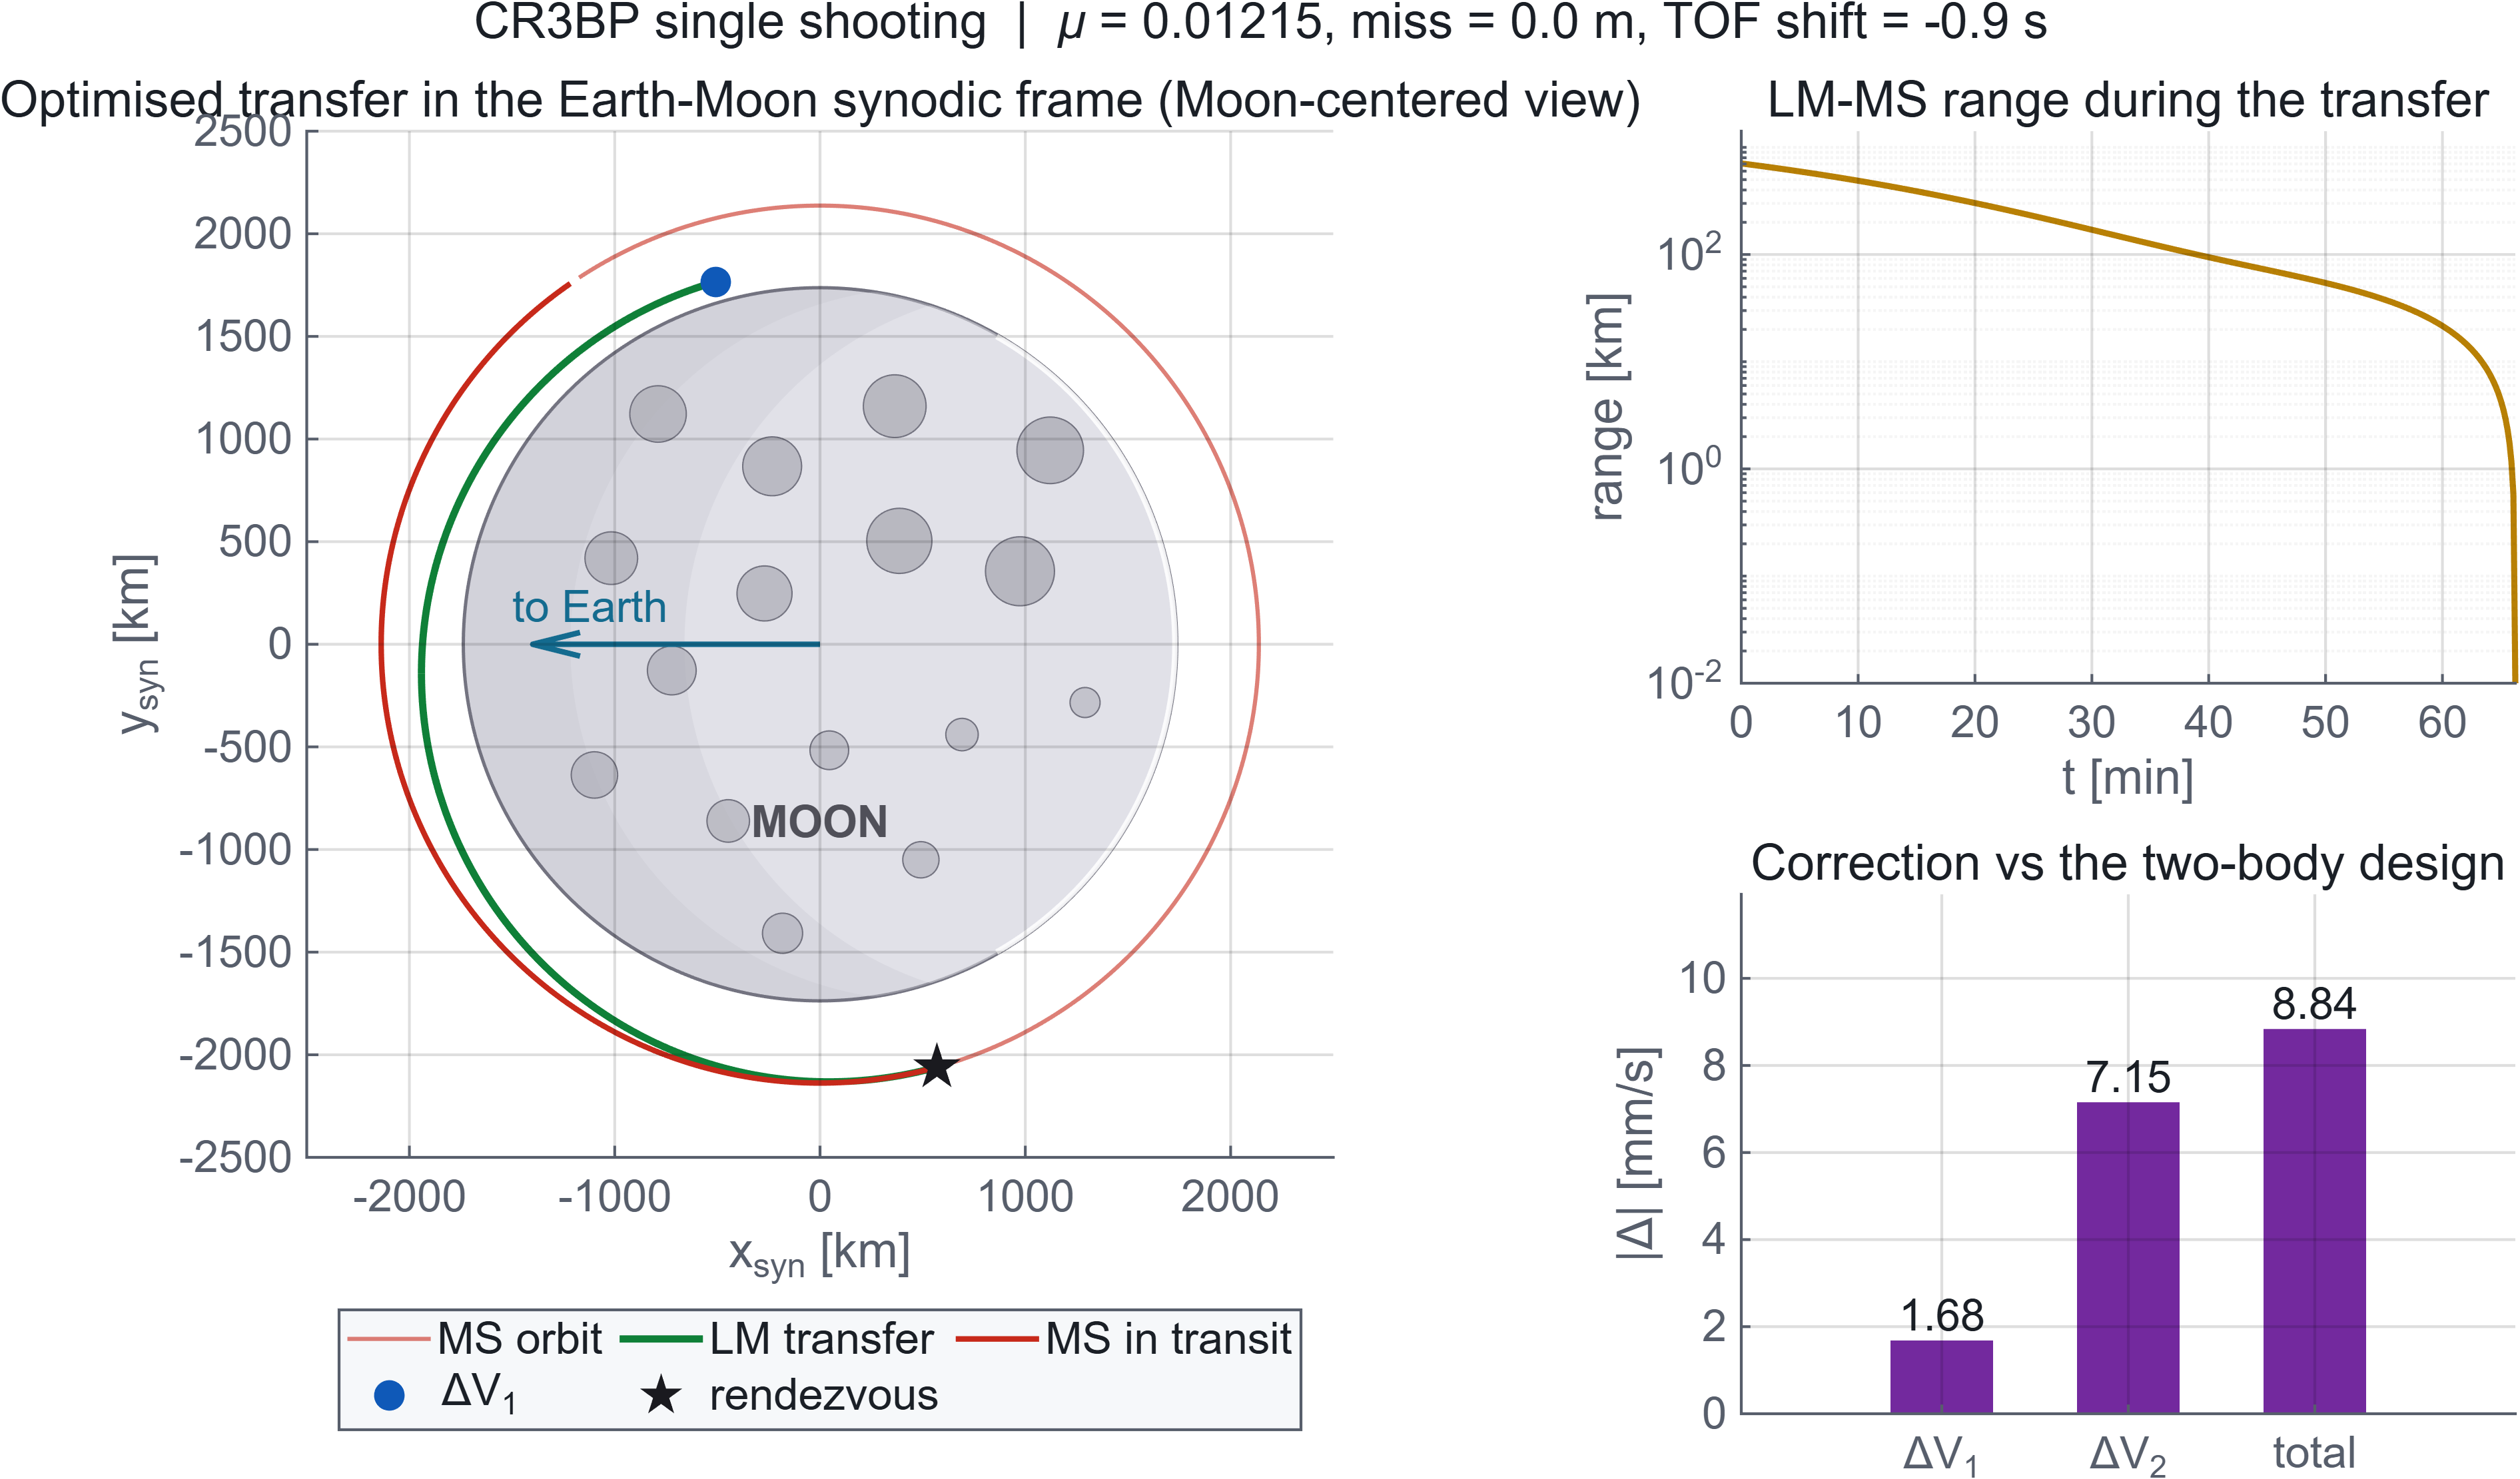
\includegraphics[width=\textwidth]{fig16_cr3bp_transfer.png}
\caption{Optimised transfer in the Earth--Moon synodic frame, Moon-centred view.
The arc is the same climb as Figure~\ref{fig:geometry} seen from a rotating
frame. Right: range history and the correction relative to the two-body design,
in millimetres per second.}
\label{fig:cr3bp}
\end{figure}

\subsection{Verification}

The CR3BP admits no energy integral, but the Jacobi constant

\begin{equation}
C_J = 2\left[\frac{x^2+y^2}{2} + \frac{1-\mu}{r_1} + \frac{\mu}{r_2}\right] - v^2
\label{eq:jacobi}
\end{equation}

is exactly conserved along any ballistic arc. Evaluated along the optimised
transfer it drifts by $9\times10^{-13}$ relative, a pure measure of integration
quality that is independent of every other check in this report.

The frame conversion is verified by the three cases listed above, and the
round trip inertial $\to$ synodic $\to$ inertial closes to $10^{-11}$.

\clearpage
\section{Berthing manipulator: kinematics and kineto-statics}
\label{sec:robotics}

\subsection{From docking to berthing}

Section~\ref{sec:proximity} delivered the chaser to the docking port with a
residual velocity of zero. In practice the last metres of a crewed vehicle's
arrival are frequently handled by a manipulator rather than by thrusters:
berthing removes the closing-rate risk, avoids plume impingement on the target,
and allows the capture to be aborted at any instant. This part characterises a
five-revolute arm sized for that job.

\subsection{Mobility}

The arm has five revolute joints connecting six bodies including the base.
Gr\"ubler's criterion in three dimensions gives

\begin{equation}
\text{DOF} = 6(N - 1 - J) + \sum_{i=1}^{J} f_i = 6(6-1-5) + 5 = 5,
\label{eq:grubler}
\end{equation}

so the arm alone has five degrees of freedom. Mounted on a free-flying base the
system has $5 + 6 = 11$. Three operating modes follow, and they are genuinely
different control problems: \emph{free-flying}, where the base pose is actively
held by thrusters; \emph{attitude-controlled}, where only orientation is held and
the base translates; and \emph{free-floating}, where nothing is actuated at the
base and total linear and angular momentum are conserved, so every arm motion
disturbs the carrier. This report assumes the free-flying case, which makes the
base pose a boundary condition rather than a state.

\subsection{Geometry and inertia}

Links are modelled as homogeneous cylinders of radius $R_c = 0.15\unit{m}$ with
the local $z$ axis along the link, so the centre of mass is at mid-length and

\begin{equation}
I_{zz} = \tfrac12 m R_c^2, \qquad
I_{xx} = I_{yy} = \tfrac{1}{12} m\left(3R_c^2 + L^2\right).
\label{eq:inertia}
\end{equation}

\begin{table}[htbp]
\centering
\caption{Link parameters. Total mass $\mArmMass\unit{kg}$, fully extended reach
$\mReach\unit{m}$. Joint axes are given in the local joint frame before the
joint rotation is applied.}
\label{tab:links}
\small
\begin{tabular}{crrrrc}
\toprule
Link & $m$ [kg] & $L$ [m] & $I_{xx}=I_{yy}$ [kg\,m$^2$] & $I_{zz}$ [kg\,m$^2$] & axis \\
\midrule
1 & $30$  & $0.60$ & $1.07$  & $0.34$ & $z$ \\
2 & $100$ & $3.20$ & $85.90$ & $1.13$ & $y$ \\
3 & $85$  & $2.80$ & $56.01$ & $0.96$ & $y$ \\
4 & $20$  & $0.60$ & $0.71$  & $0.23$ & $y$ \\
5 & $15$  & $0.50$ & $0.40$  & $0.17$ & $x$ \\
\bottomrule
\end{tabular}
\end{table}

\subsection{Forward kinematics}

Frames are placed at the link centres of mass with $z$ along the link, and
offsets are pure $z$ translations: $g_i = L_i/2$ from joint $i$ to the centre of
mass of link $i$, and $b_i = L_i/2$ from that centre of mass to joint $i+1$. The
chain is

\begin{equation}
T_i = T_{i-1}\, \mathrm{Trans}(b_{i-1})\, \mathrm{Rot}(\mathbf e_i, \theta_i)\, \mathrm{Trans}(g_i),
\label{eq:chain}
\end{equation}

with the rotation built from the Euler--Rodrigues formula

\begin{equation}
R(\mathbf e, \theta) = \cos\theta\, I + (1-\cos\theta)\,\mathbf e\mathbf e^\top + \sin\theta\,[\mathbf e\times].
\label{eq:rodrigues}
\end{equation}

The end-effector frame is one further half-link beyond the last centre of mass,
at the physical tip.

For the acceptance pose $\boldsymbol\theta = [0, 45, 0, 60, 0]^\circ$ the chain
returns a rotation of exactly $R_y(105^\circ)$ -- joints 2, 3 and 4 share the
$y$ axis, so only their sum matters -- and a tip position of
$[5.305, 0, 4.558]^\top\unit{m}$. Both reproduce the reference pose to
$6\times10^{-5}$.

\begin{figure}[htbp]
\centering
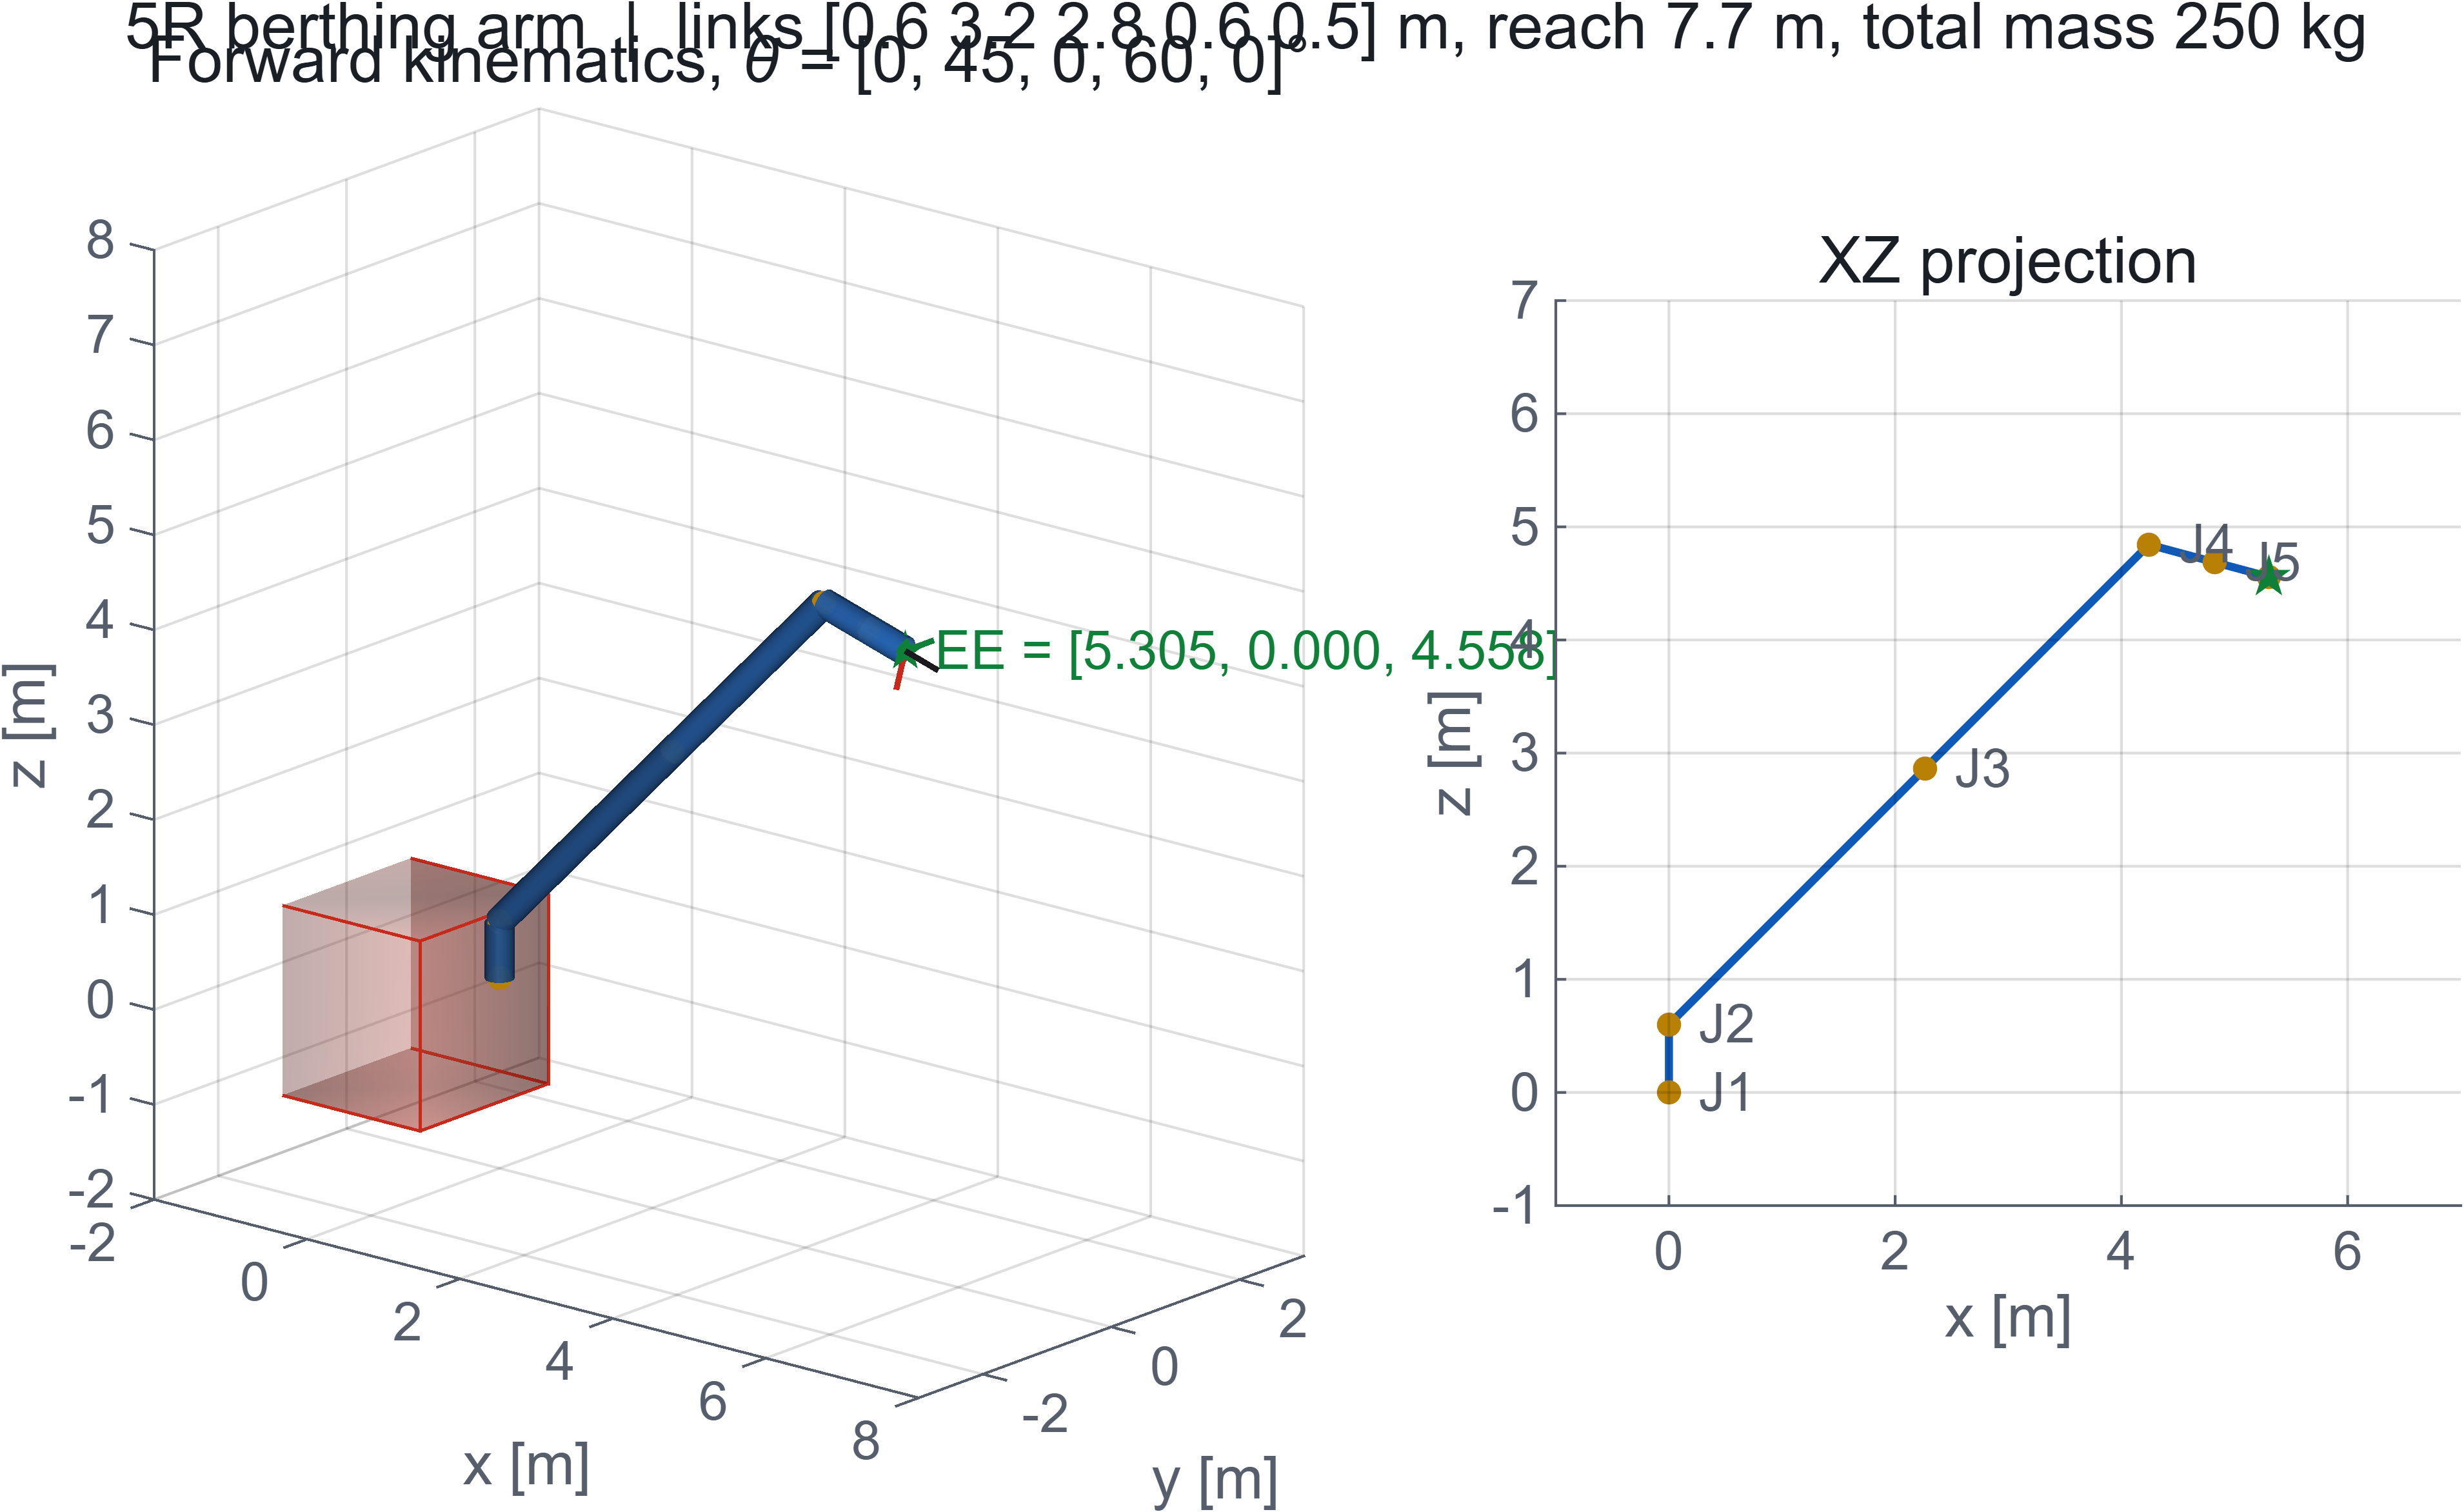
\includegraphics[width=\textwidth]{fig14_fkine_verification.png}
\caption{Forward kinematics at the acceptance pose. Left: three-dimensional
rendering with the end-effector triad. Right: $xz$ projection with the joint
origins labelled. Reach at this pose is $6.99\unit{m}$ of the $\mReach\unit{m}$
maximum.}
\label{fig:fk}
\end{figure}

\subsection{Twist propagation and kineto-static duality}

Velocities are propagated with a system Jacobian mapping the eleven generalised
velocities to the six body twists,

\begin{equation}
\mathbf t = N\,\mathbf u, \qquad
\mathbf u = \begin{bmatrix}\boldsymbol\omega_0 \\ \dot{\mathbf r}_0 \\ \dot{\mathbf q}\end{bmatrix} \in \mathbb{R}^{11},
\qquad \mathbf t \in \mathbb{R}^{36},
\qquad N = N_l N_d .
\label{eq:N}
\end{equation}

Here $N_d = \mathrm{blkdiag}(I_6, \mathbf p_1, \dots, \mathbf p_5)$ injects each
joint rate into its own body with
$\mathbf p_i = [\mathbf e_i;\ \mathbf e_i\times\mathbf g_i]$ in inertial axes,
and $N_l$ is block lower triangular with unit diagonal and rigid-body transports

\begin{equation}
B_{ij} = \begin{bmatrix} I_3 & 0 \\ [(\mathbf r_j - \mathbf r_i)\times] & I_3 \end{bmatrix}.
\label{eq:transport}
\end{equation}

The sign is the part worth checking: $\mathbf v_i = \mathbf v_j + \boldsymbol\omega_j\times(\mathbf r_i - \mathbf r_j)$
and $\boldsymbol\omega_j\times\mathbf d = -[\mathbf d\times]\boldsymbol\omega_j$,
hence $[(\mathbf r_j - \mathbf r_i)\times]$ and not the reverse. Getting it
backwards produces a base reaction whose force is right and whose moment is
wrong -- a failure mode that no plot reveals and that the tests of
Section~\ref{sec:robotics:verif} catch immediately.

In micro-gravity with a single external wrench at the end effector, static
equilibrium gives the generalised forces by duality,

\begin{equation}
\boldsymbol\tau = N^\top \mathbf w,
\label{eq:duality}
\end{equation}

where $\mathbf w$ stacks the body wrenches ordered $[\text{moment};\text{force}]$
to match the $[\boldsymbol\omega; \mathbf v]$ twist ordering. Only the last body
is loaded, with the contact wrench transported from the tip to the centre of
mass of link 5. The actuators and the attitude control system must supply
$-\boldsymbol\tau$.

\subsection{Load cases}

Two contact wrenches are applied at three postures: a purely axial
$\mathbf F = [0,0,-100]^\top\unit{N}$ representing a nominal berthing push, and a
misaligned $\mathbf F = [15,-10,-80]^\top\unit{N}$ with
$\mathbf M = [12,8,-5]^\top\unit{N\,m}$ representing an off-nominal capture.

\begin{table}[htbp]
\centering
\caption{Joint torques [N\,m] under the $100\unit{N}$ axial berthing load. The
base reaction force is $100.00\unit{N}$ in every case, as a static chain loaded
by a single external force requires.}
\label{tab:torque1}
\small
\begin{tabular}{lrrrrrr}
\toprule
Posture & $\tau_1$ & $\tau_2$ & $\tau_3$ & $\tau_4$ & $\tau_5$ & $\lVert\mathbf n_{\text{base}}\rVert$ \\
\midrule
Nearly extended & $0.00$   & $79.97$   & $24.40$   & $0.00$  & $0.00$ & $79.97$ \\
Folded          & $0.00$   & $396.47$  & $95.77$   & $0.00$  & $0.00$ & $435.03$ \\
General spatial & $131.18$ & $-339.41$ & $-194.40$ & $0.00$  & $0.00$ & $486.30$ \\
\bottomrule
\end{tabular}
\end{table}

\begin{table}[htbp]
\centering
\caption{Joint torques [N\,m] under the misaligned wrench. Base reaction force
$82.01\unit{N}$ throughout. Note that $\tau_1$ and $\tau_5$, identically zero in
the axial case, are now loaded.}
\label{tab:torque2}
\small
\begin{tabular}{lrrrrrr}
\toprule
Posture & $\tau_1$ & $\tau_2$ & $\tau_3$ & $\tau_4$ & $\tau_5$ & $\lVert\mathbf n_{\text{base}}\rVert$ \\
\midrule
Nearly extended & $-13.00$ & $177.59$  & $85.86$   & $24.50$ & $17.00$ & $206.88$ \\
Folded          & $-9.54$  & $364.72$  & $140.58$  & $24.50$ & $17.00$ & $407.65$ \\
General spatial & $62.26$  & $-193.62$ & $-112.42$ & $25.16$ & $17.00$ & $279.64$ \\
\bottomrule
\end{tabular}
\end{table}

Four observations follow, and they are the engineering content of the tables.

\begin{itemize}
\item With the arm nearly extended and the load axial, the force runs along the
      links. The $y$-axis joints see a short moment arm and the shoulder carries
      only $80\unit{N\,m}$.
\item Folding the arm turns the same $100\unit{N}$ into a long transverse lever
      and the shoulder torque rises to $\mTauMax\unit{N\,m}$, the largest value
      in the study. Actuator sizing is driven by posture, not by load magnitude.
\item The axial load leaves the base turret ($\tau_1$) and the wrist roll
      ($\tau_5$) at exactly zero, because their axes are parallel to the force or
      pass through its line of action. The misaligned wrench activates both.
      A capture mechanism designed only for the nominal case would under-size
      precisely these two actuators.
\item Masses appear nowhere in either table. In micro-gravity the static problem
      is mass-free; the inertias of Table~\ref{tab:links} would enter the mass
      matrix and Coriolis terms of the free-floating dynamics, which this report
      does not integrate.
\end{itemize}

\begin{figure}[htbp]
\centering
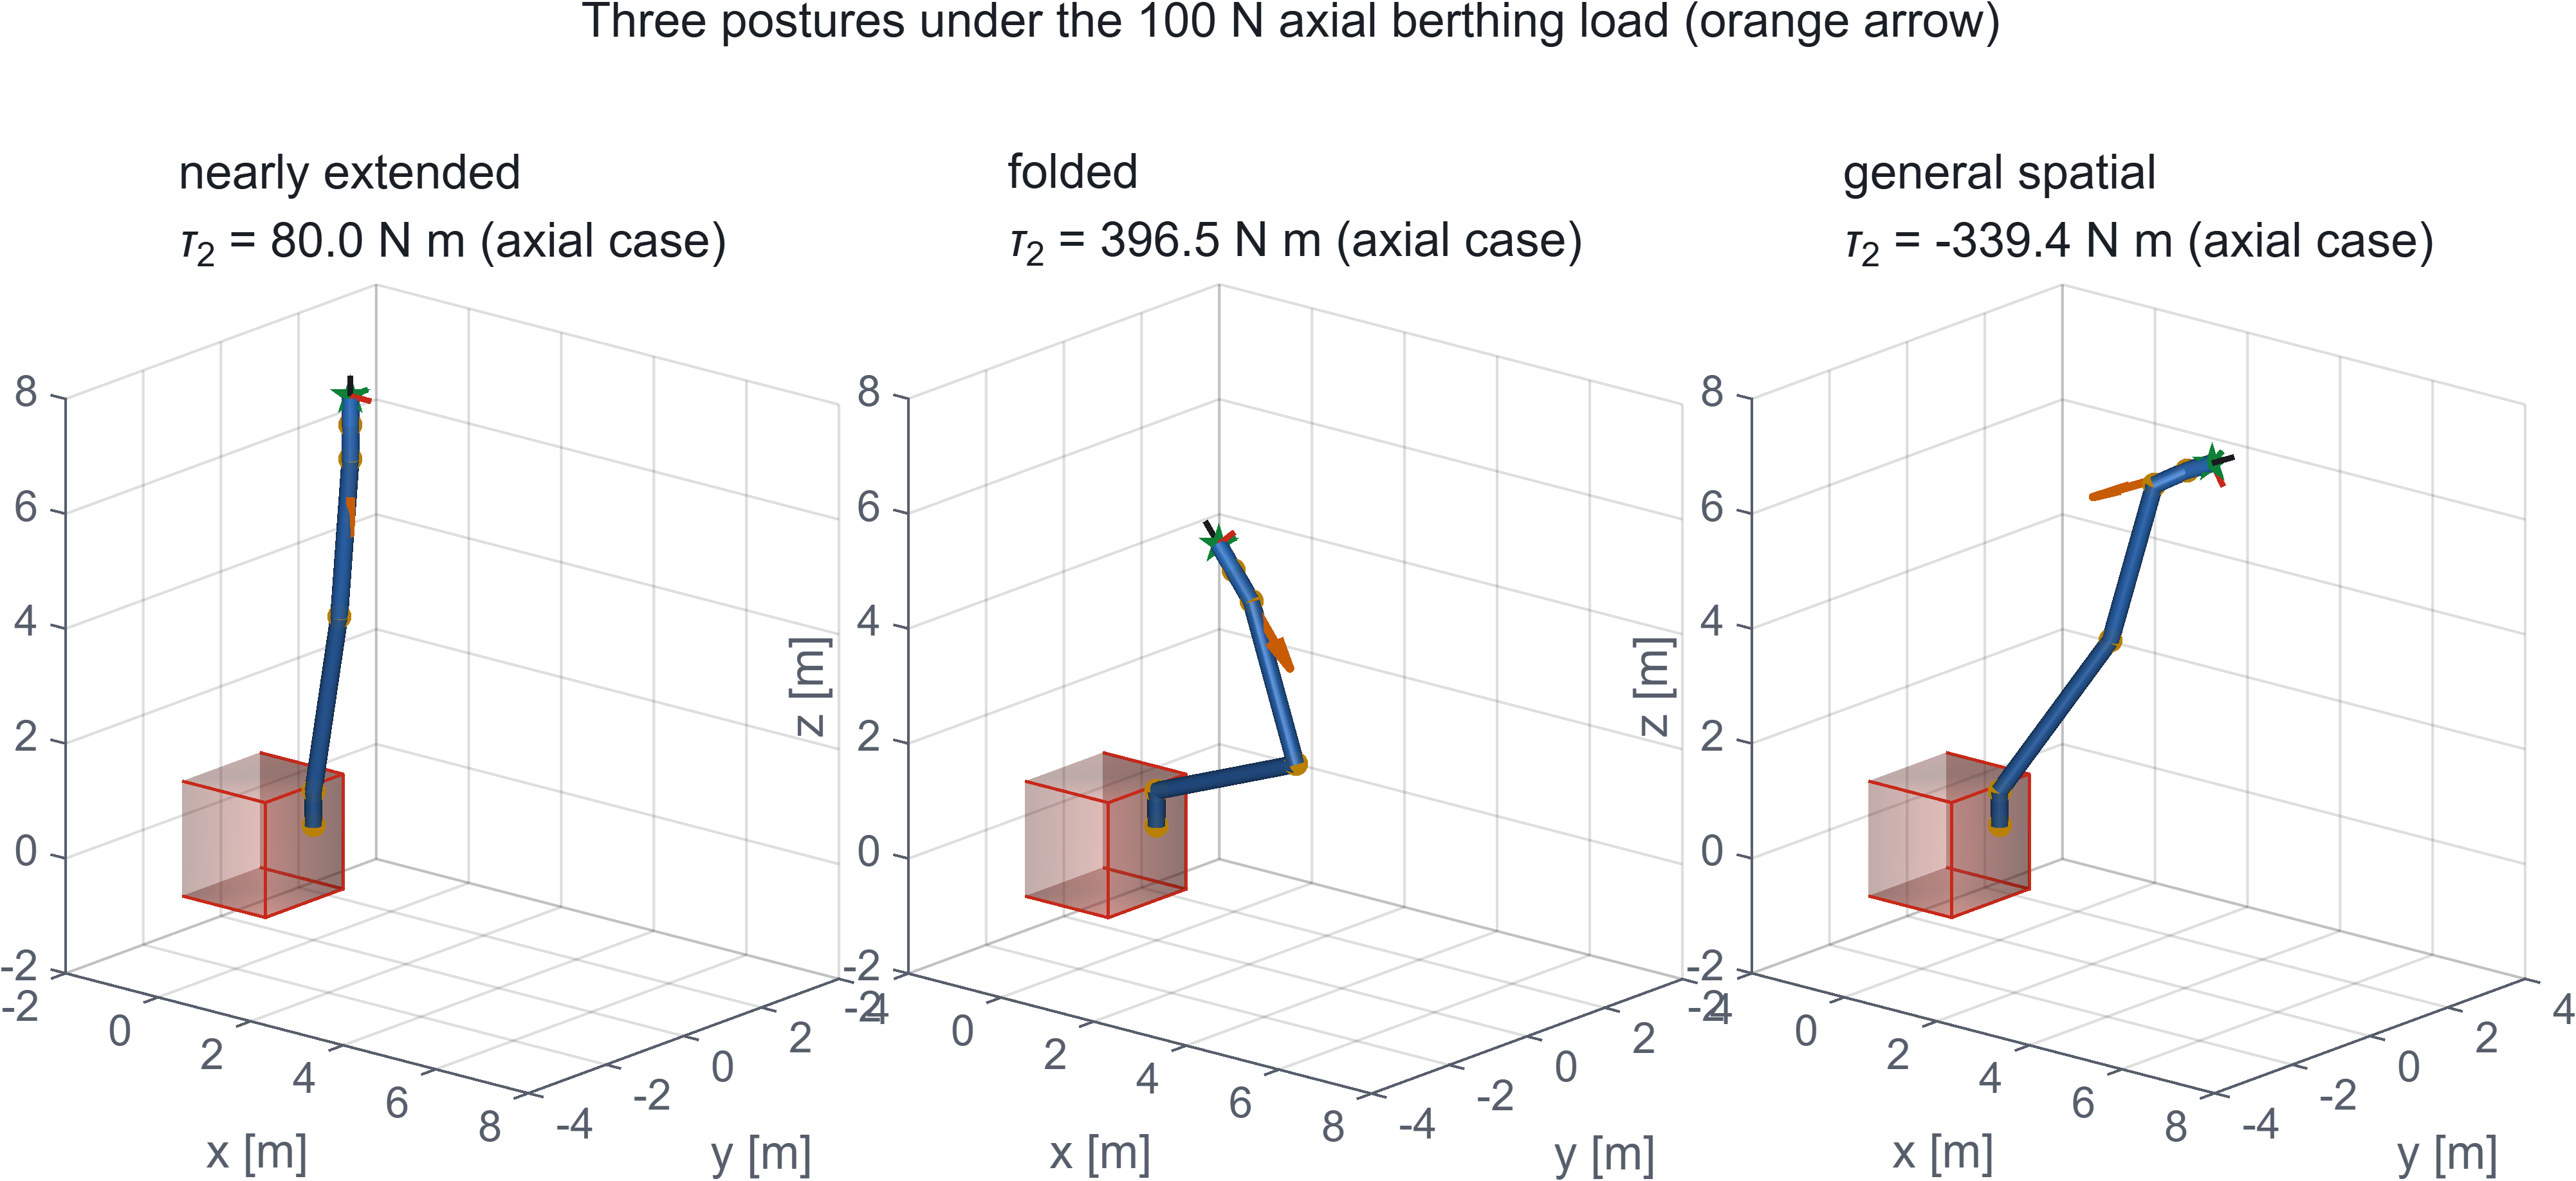
\includegraphics[width=\textwidth]{fig15_three_postures.png}
\caption{The three study postures under the $100\unit{N}$ axial berthing load
(arrow). Shoulder torque rises fivefold from the extended to the folded
configuration for an identical applied force.}
\label{fig:postures}
\end{figure}

\subsection{Verification}
\label{sec:robotics:verif}

Two statements must hold for a static chain loaded by a single external wrench,
and both are tested at every posture and load case:

\begin{enumerate}[label=(\roman*)]
\item the force part of the base reaction equals the applied force exactly, and
      the moment part equals $\mathbf M_{\text{tip}} + (\mathbf r_{\text{tip}} - \mathbf r_{\text{base}})\times\mathbf F$;
\item the joint torques obtained from the $36\times11$ twist-propagation route
      equal those obtained from the $6\times5$ end-effector Jacobian,
      $\boldsymbol\tau_m = J^\top[\mathbf f; \mathbf n]$.
\end{enumerate}

The worst residuals are $2\times10^{-14}\unit{N}$ and $\mDualRes\unit{N\,m}$.
Two entirely different pieces of algebra agreeing to machine precision is
stronger evidence than either one looking plausible on its own.

\clearpage
\section{Inverse kinematics and the capture manoeuvre}
\label{sec:ik}

\subsection{A five-joint arm in a six-dimensional task space}

The manipulator has five joints; a rigid-body pose has six degrees of freedom.
The pose problem is therefore structurally unsolvable in general, and a solver
that hides this fact by converging to something is worse than one that does not
converge. The approach taken here states the deficiency in the weighting and
reports the residual it leaves.

\subsection{Spatial error}

Given a target pose $(\mathbf p_t, R_t)$ and the current pose
$(\mathbf p_k, R_k)$ with columns $\mathbf x_k, \mathbf y_k, \mathbf z_k$, the
task error is

\begin{equation}
\Delta\mathbf p = \mathbf p_t - \mathbf p_k, \qquad
\mathbf e_o = \tfrac12\left(\mathbf x_k\times\mathbf x_t + \mathbf y_k\times\mathbf y_t + \mathbf z_k\times\mathbf z_t\right),
\qquad
\Delta\mathbf x = \begin{bmatrix}\Delta\mathbf p \\ \mathbf e_o\end{bmatrix}.
\label{eq:taskerr}
\end{equation}

The orientation error uses the Siciliano form \cite{siciliano} rather than
axis-angle extraction, which is singular at $\pm180^\circ$. That is not a
theoretical concern here: the seeds used are far from the target and rotations
near $180^\circ$ genuinely occur on the first iterations.

\subsection{Weighted damped least squares}

The geometric Jacobian is assembled column by column for revolute joints,

\begin{equation}
J_i = \begin{bmatrix} \mathbf z_{i}\times(\mathbf p_{EE} - \mathbf r_{i}) \\ \mathbf z_{i}\end{bmatrix},
\label{eq:jacobian}
\end{equation}

ordered $[\text{linear};\text{angular}]$ to match~\eqref{eq:taskerr}, and the
update is

\begin{equation}
\boldsymbol\theta \leftarrow \boldsymbol\theta + \alpha\left(J^\top W J + \lambda^2 I\right)^{-1} J^\top W \Delta\mathbf x,
\label{eq:wdls}
\end{equation}

with $\lambda = 0.05$, $\alpha = 0.4$ and
$W = \mathrm{diag}(1,1,1,1,1,0.01)$. The damping keeps the update bounded near
singular configurations; the weighting spends the available freedom on position
and de-emphasises the one attitude component a five-joint wrist cannot serve.

\subsection{A real singularity at the obvious seed}

The stowed configuration $\boldsymbol\theta = \mathbf 0$ is not a neutral
starting point. Fully extended along $z$, joint~1 rotates about an axis passing
through the end effector, so it produces no end-effector translation at all and
the position Jacobian loses a column. The solver escapes because the attitude
term still torques joint~1, but the code carries a deterministic seed cascade
anyway and logs which seed was used, rather than pretending the singularity is
not there.

\subsection{Results}

Two targets are run. The first is the forward-kinematics pose of a known
configuration, so an exact solution provably exists and the convergence claim
means something. Starting from the zero pose the solver reaches
$\mIKres\unit{mm}$ in $\mIKiters$ iterations, well inside the $80$-iteration
budget.

The solution found is \emph{not} the configuration the target was generated
from: the solver returns $[40.0, 16.3, 20.1, 28.6, 25.0]^\circ$ against the
generating $[40, 35, -20, 50, 25]^\circ$. Both reach the same pose because
joints 2, 3 and 4 rotate about a common axis and only their sum enters -- $65^\circ$
in both cases. Multiple inverse solutions are the expected behaviour of a serial
chain, not a defect.

The second target is operationally motivated: a point $0.4\unit{m}$ in front of
the mothership docking face with the tool axis along $+x$. Position converges to
$\mIKtwoRes\unit{mm}$ and a small attitude residual survives, which is precisely
the structural deficiency admitted at the start of this section.

\begin{figure}[htbp]
\centering
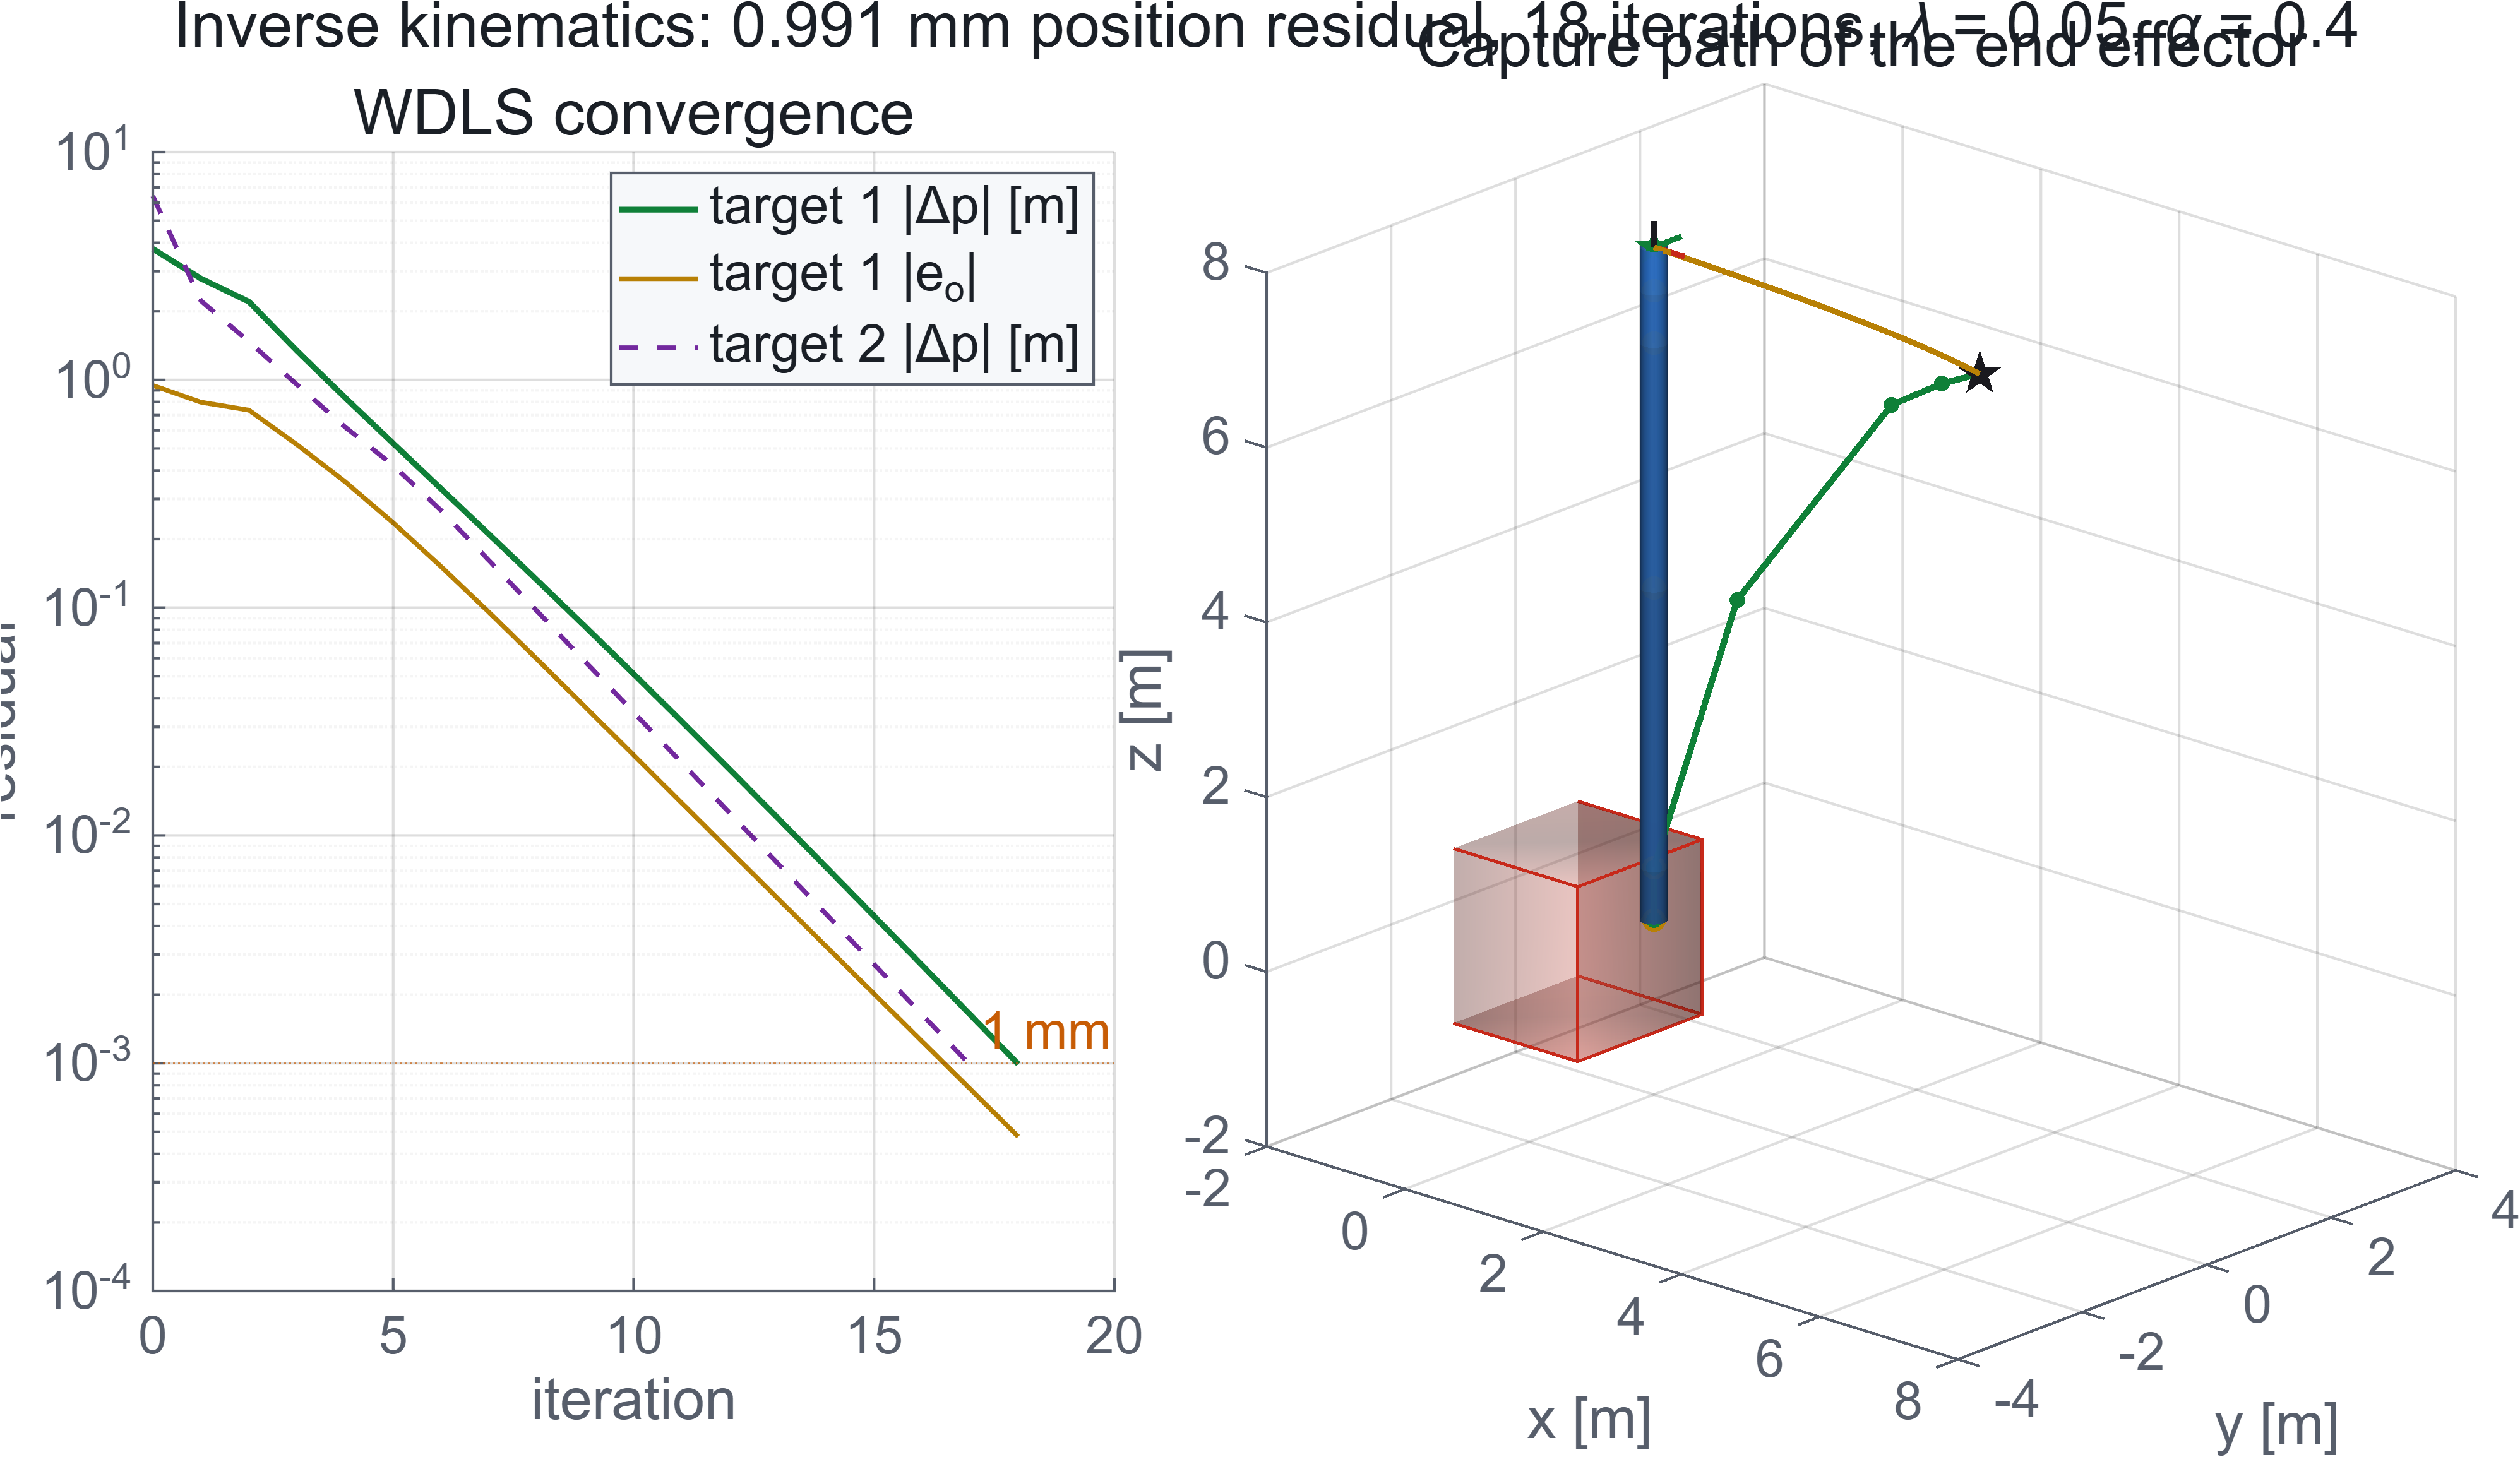
\includegraphics[width=\textwidth]{fig20_ik_convergence.png}
\caption{Left: WDLS convergence for both targets, log scale. Position residual
falls below $1\unit{mm}$ in $\mIKiters$ iterations. Right: the capture path of
the end effector from the stowed pose to the solution, with the final
configuration overlaid.}
\label{fig:ik}
\end{figure}

\subsection{Rest-to-rest joint trajectory}

The capture is flown as a cubic in joint space over $t_f = 30\unit{s}$ with zero
rate at both ends,

\begin{equation}
\theta(t) = \theta_0 + \frac{3\Delta\theta}{t_f^2}t^2 - \frac{2\Delta\theta}{t_f^3}t^3,
\qquad
\dot\theta(t) = \frac{6\Delta\theta}{t_f^2}t - \frac{6\Delta\theta}{t_f^3}t^2 .
\label{eq:cubic}
\end{equation}

A cubic rather than a quintic is a deliberate choice: berthing rates are slow
enough that the discontinuous acceleration at the endpoints is harmless, and the
velocity profile stays trivially verifiable. The peak rate is
$1.5\,\Delta\theta/t_f$ at mid-time, here $0.035\unit{rad/s}$, and the end
effector travels $4.12\unit{m}$ along the capture path.

\begin{figure}[htbp]
\centering
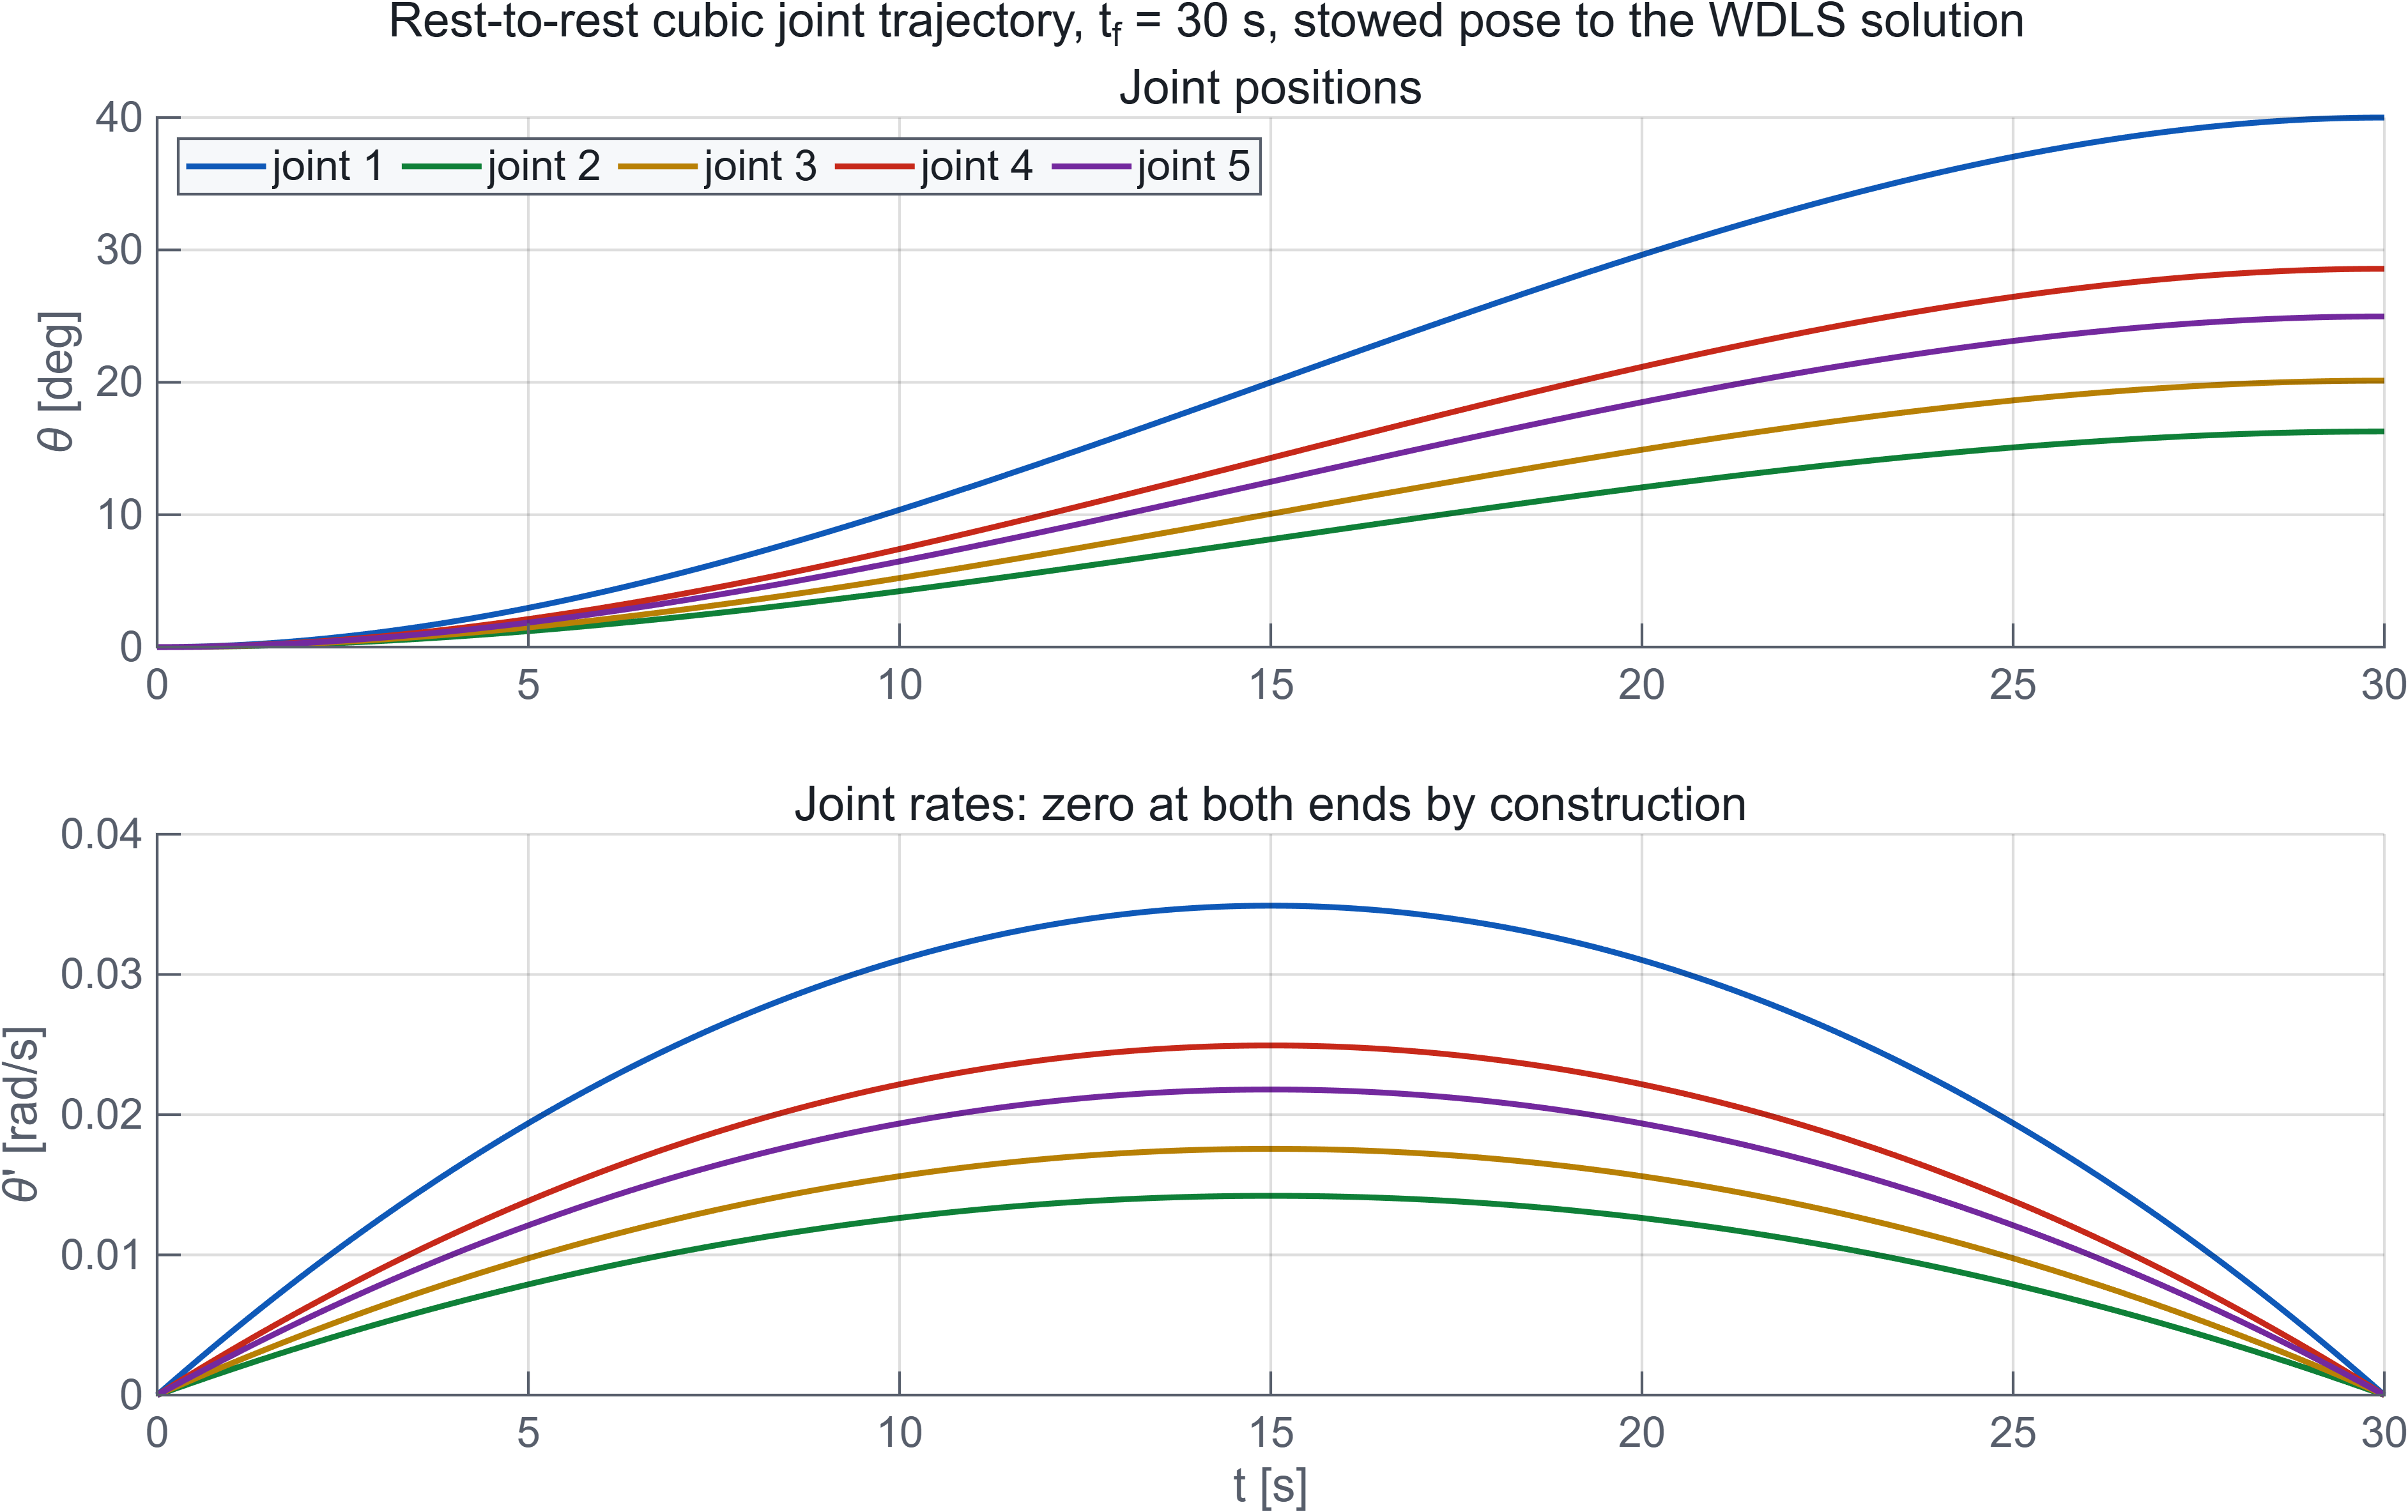
\includegraphics[width=0.95\textwidth]{fig17_joint_trajectory.png}
\caption{Rest-to-rest cubic joint trajectory over $30\unit{s}$. Rates start and
end at exactly zero, which is checked to $10^{-17}\unit{rad/s}$ rather than read
off the plot.}
\label{fig:cubic}
\end{figure}

\subsection{Verification}

The boundary conditions of~\eqref{eq:cubic} are checked symbolically against the
sampled trajectory: $\theta(0) = \theta_0$ and $\theta(t_f) = \theta^*$ to
$10^{-16}$, $\dot\theta(0) = \dot\theta(t_f) = 0$ to $10^{-17}$, and the peak
rate matches the analytical $1.5\Delta\theta/t_f$ exactly. The inverse-kinematics
solution is verified the only way that is meaningful for an iterative solver: by
pushing the returned joint vector back through the forward kinematics of
Section~\ref{sec:robotics} and measuring the pose it actually produces.

\clearpage
\section{Discussion}
\label{sec:discussion}

\subsection{Consolidated results}

\begin{table}[htbp]
\centering
\caption{Headline results. Every value is read from the simulation output at
compile time, so this table cannot drift out of step with the code.}
\label{tab:summary}
\small
\begin{tabular}{llr}
\toprule
Phase & Quantity & Value \\
\midrule
Transfer   & Total impulsive $\dv$              & $\mDVtot\unit{m/s}$ \\
           & Phasing wait                       & $\mTwaitH\unit{h}$ \\
           & Mission duration                   & $\mTmissionH\unit{h}$ \\
           & Numerical vs analytical error      & $\mKeplerErrMm\unit{mm}$ \\
\midrule
Proximity  & Injection error                    & $\mDrZero\unit{m}$, $\mDvZero\unit{m/s}$ \\
           & Uncorrected drift, 3 orbits        & $\mDriftKm\unit{km}$ \\
           & Hold acquisition $\dv$             & $\mDVhold\unit{m/s}$ \\
           & Docking $\dv$                      & $\mDVdock\unit{m/s}$ \\
           & Linearisation error, 3 orbits      & $\mNlSep\unit{m}$ \\
\midrule
Perturbed  & $J_2$ miss, no retargeting         & $\mMissJtwo\unit{km}$ \\
           & Third-body contribution            & $\mMissTB\unit{m}$ \\
           & Mid-course correction budget       & $\mDVmcc\unit{m/s}$ \\
\midrule
CR3BP      & Converged miss                     & $\mCRmiss\unit{m}$ \\
           & Correction to the two-body design  & $\mCRextra\unit{mm/s}$ \\
\midrule
Robotics   & Reach, 5R                          & $\mReach\unit{m}$ \\
           & Peak joint torque at $100\unit{N}$ & $\mTauMax\unit{N\,m}$ \\
           & IK position residual               & $\mIKres\unit{mm}$ in $\mIKiters$ iterations \\
\bottomrule
\end{tabular}
\end{table}

\subsection{Verification summary, including what disagrees}
\label{sec:discussion:verif}

An automated audit re-derives every design scalar in closed form from the raw
constants and compares the rest against an independent implementation of the
same mission geometry. It records $60$ passes, one warning and no failures. The
three results worth discussing are the ones that did not match exactly.

\paragraph{Docking $\dv$: $\mDVdock$ against $0.1567\unit{m/s}$ ($0.02\%$).}
The forced \vbar{} profile is almost pure geometry, so agreement at this level
means the leg targeting, waypoint spacing and braking impulse are modelled
identically. This is the strongest single confirmation that the proximity module
is faithful.

\paragraph{Third body: $\mMissTB$ against $116.0\unit{m}$ ($0.2\%$).}
Agreement at this level on a $116\unit{m}$ effect tests two things that are easy
to get wrong: the retention of the indirect term in~\eqref{eq:thirdbody}, and
the use of the synodic rate for the Earth ephemeris. Dropping the indirect term
inflates the number by orders of magnitude, so a match this tight is real
evidence rather than a coincidence.

\paragraph{$J_2$ miss: $\mMissJtwo\unit{km}$ against $14.56\unit{km}$ ($+4\%$).}
The four plausible causes were checked in the source rather than assumed: the
departure impulse is applied along the perturbed velocity, the target is
propagated with the same perturbed dynamics as the chaser, the full
three-component $J_2$ formula is used, and the Keplerian control case through
the identical code path closes to $5.6\times10^{-3}\unit{m}$. None is at fault.
The residual is sensitivity, not error. The miss is a \emph{difference} of two
nearly equal secular phase slips accumulated over ten and a half hours, so it
inherits the sensitivity of both to the exact burn epoch and to the integrator
tolerance. Two correct implementations agreeing to $4\%$ on such a quantity is
the expected outcome, and the discrepancy was documented rather than removed.

\paragraph{CR3BP correction: $\mCRextra\unit{mm/s}$ against $1.5\unit{mm/s}$.}
The single warning. As explained in Section~\ref{sec:cr3bp}, the planar shooting
problem is rank-deficient by one, so the zero-miss set is a curve and different
optimiser starts land at different points on it. Both figures support the same
operational statement -- Earth tides move this budget by millimetres per second
-- and forcing agreement would be curve-fitting rather than physics.

\paragraph{Hold $\dv$: $\mDVhold$ against $1.4\unit{m/s}$.}
Not comparable: the injection error is a random draw and the two runs use
different realisations. Fed the reference draw, our targeting returns
$1.419\unit{m/s}$, reproducing the reference to $1.4\%$. That test is also what
settles the frame convention of Section~\ref{sec:proximity:frame}.

\subsection{Limitations}
\label{sec:limits}

This is an engineering-faithful simulation of a restricted model. The following
would each change a specific number, and are named so that no reader has to
discover them.

\begin{itemize}
\item \textbf{Equatorial, coplanar orbits only.} No inclination difference and no
      relative right ascension, so the out-of-plane budget that dominates real
      rendezvous planning never appears. This is the single largest omission.
\item \textbf{Gravity stops at $J_2$.} The real lunar field is dominated by mass
      concentrations rather than a clean oblateness term \cite{zuber_grail}, and
      the $C_{22}$ ellipticity is comparable to $J_2$ for some geometries. Low
      lunar orbits are genuinely unstable over weeks under the true field.
      Nothing here runs that long, but the frozen-orbit design a real mission
      would use is a numerical search this model cannot support.
\item \textbf{No solar radiation pressure.} Estimated at $10^{-7}\unit{m/s^2}$
      and excluded with the reasoning given in Section~\ref{sec:perturbations};
      the flag exists but no cannonball model is wired in.
\item \textbf{Impulsive burns.} Finite-burn losses, throttle profiles, attitude
      slews and propellant slosh are all absent. For a $60\unit{m/s}$ impulse the
      gravity loss is small, but it is not zero.
\item \textbf{Circular target orbit, not a halo.} A realistic Artemis-era
      architecture places the mothership in a near-rectilinear halo orbit, where
      the rendezvous geometry and the phasing analysis are qualitatively
      different problems.
\item \textbf{The arm is kinematic and static.} Five degrees of freedom, a base
      held fixed by assumption, no joint flexibility, no contact dynamics, and no
      free-floating momentum coupling. The local frame is treated as inertial
      during berthing.
\item \textbf{One random draw.} The injection error is a single realisation, not
      a Monte Carlo campaign. The proximity $\dv$ figures are therefore one
      sample of a distribution whose spread is not characterised.
\end{itemize}

\subsection{Conclusions}

Three results are worth carrying away.

First, the propellant cost of this return phase is dominated by the transfer,
not by the corrections: $\mDVtot\unit{m/s}$ for the Hohmann climb against
$\mDVprox\unit{m/s}$ for all proximity operations, roughly $1\%$. What the
ascent dispersion actually costs is small, provided it is corrected early.

Second, the binding constraint is time, not propellant. The transfer lasts
$66$ minutes; waiting for the phasing window takes $\mTwaitH$ hours. Any
architecture that needs a fast return has to buy it with a non-Hohmann transfer,
and the CR3BP analysis shows that the extra energy will not come from
three-body effects at this altitude.

Third, the perturbation that matters at $100$--$400\unit{km}$ is lunar
oblateness, not the Earth. $J_2$ displaces the meeting point by
$\mMissJtwo\unit{km}$ and demands a $\mDVmcc\unit{m/s}$ mid-course correction;
the Earth contributes $\mMissTB\unit{m}$ and the full three-body treatment
changes the budget by $\mCRextra\unit{mm/s}$. Effort spent modelling the Earth
here is effort not spent on the lunar field, which is the opposite of the
intuition one brings from Earth orbit.

\subsection{Reproducibility}

The complete simulation runs unattended from a single command and takes about
ten minutes, of which roughly one is physics and the rest is rendering. It
requires base MATLAB only: no toolbox, no external ephemeris, no downloaded
imagery. All results in this report, including every figure, were produced by
the run whose audit table is reproduced in the repository as
\texttt{results/AUDIT\_REPORT.md}.


\bibliographystyle{plain}
\bibliography{refs}

\end{document}
